% Gerbrich Ferdinands, research report 20.12.2019
% adapted from the BMC bioinformatics .tex template (https://bmcbioinformatics.biomedcentral.com/submission-guidelines/preparing-your-manuscript)

 
%% BioMed_Central_Tex_Template_v1.06
%%                                      %
%  bmc_article.tex            ver: 1.06 %
%                                       %

%%IMPORTANT: do not delete the first line of this template
%%It must be present to enable the BMC Submission system to
%%recognise this template!!

%%%%%%%%%%%%%%%%%%%%%%%%%%%%%%%%%%%%%%%%%
%%                                     %%
%%  LaTeX template for BioMed Central  %%
%%     journal article submissions     %%
%%                                     %%
%%          <8 June 2012>              %%
%%                                     %%
%%                                     %%
%%%%%%%%%%%%%%%%%%%%%%%%%%%%%%%%%%%%%%%%%


%%%%%%%%%%%%%%%%%%%%%%%%%%%%%%%%%%%%%%%%%%%%%%%%%%%%%%%%%%%%%%%%%%%%%
%%                                                                 %%
%% For instructions on how to fill out this Tex template           %%
%% document please refer to Readme.html and the instructions for   %%
%% authors page on the biomed central website                      %%
%% http://www.biomedcentral.com/info/authors/                      %%
%%                                                                 %%
%% Please do not use \input{...} to include other tex files.       %%
%% Submit your LaTeX manuscript as one .tex document.              %%
%%                                                                 %%
%% All additional figures and files should be attached             %%
%% separately and not embedded in the \TeX\ document itself.       %%
%%                                                                 %%
%% BioMed Central currently use the MikTex distribution of         %%Ffjdk
%% TeX for Windows) of TeX and LaTeX.  This is available from      %%
%% http://www.miktex.org                                           %%
%%                                                                 %%
%%%%%%%%%%%%%%%%%%%%%%%%%%%%%%%%%%%%%%%%%%%%%%%%%%%%%%%%%%%%%%%%%%%%%

%%% additional documentclass options:
%  [doublespacing]
%  [linenumbers]   ; put the line numbers on margins

%%% loading packages, author definitions

\documentclass[twocolumn]{bmcart}% uncomment this for twocolumn layout and comment line below
%\documentclass{bmcart}
%%% Load packages–≠
\usepackage{amsthm,amsmath}
\usepackage{listings}
%\usepackage[lofdepth,lotdepth]{subfig}
\usepackage{subfigure}

%\RequirePackage{}
%\RequirePackage[authoryear]{natbib}% uncomment this for author;year bibliography
\RequirePackage{hyperref}
%\RequirePackage{natbib}
\usepackage[utf8]{inputenc} %unicode support
%\usepackage[applemac]{inputenc} %applemac support if unicode package fails
%\usepackage[latin1]{inputenc} %UNIX support if unicode package fails
\usepackage{xcolor}
\usepackage{graphicx} %package to manage images
\graphicspath{ {./images/} }%Path relative to the main .tex file 
%\usepackage{subcaption}
\usepackage{multicol}
%New colors defined below
\definecolor{codegreen}{rgb}{0,0.6,0}
\definecolor{codegray}{rgb}{0.5,0.5,0.5}
\definecolor{codepurple}{rgb}{0.58,0,0.82}
\definecolor{backcolour}{rgb}{0.95,0.95,0.92}

%Code listing style named "mystyle"
\lstdefinestyle{mystyle}{
  backgroundcolor=\color{backcolour},   commentstyle=\color{codegreen},
  % keywordstyle=\color{magenta},
  numberstyle=\tiny\color{codegray},
  stringstyle=\color{codepurple},
  basicstyle=\ttfamily\footnotesize,
  breakatwhitespace=false,         
  breaklines=true,                 
  captionpos=b,                    
  keepspaces=true,                 
  %numbers=left,                    
  %numbersep=5pt,                  
  showspaces=false,                
  showstringspaces=false,
  showtabs=false,                  
  tabsize=2
}
\newcommand{\irow}[1]{% inline row vector
  \begin{smallmatrix}(#1)\end{smallmatrix}%
}

\lstset{style=mystyle}
\usepackage{setspace}
%%%%%%%%%%%%%%%%%%%%%%%%%%%%%%%%%%%%%%%%%%%%%%%%%
%%                                             %%
%%  If you wish to display your graphics for   %%
%%  your own use using includegraphic or       %%
%%  includegraphics, then comment out the      %%
%%  following two lines of code.               %%
%%  NB: These line *must* be included when     %%
%%  submitting to BMC.                         %%
%%  All figure files must be submitted as      %%
%%  separate graphics through the BMC          %%
%%  submission process, not included in the    %%
%%  submitted article.                         %%
%%                                             %%
%%%%%%%%%%%%%%%%%%%%%%%%%%%%%%%%%%%%%%%%%%%%%%%%%

%\def\includegraphic{}
%\def\includegraphics{}

%%% Put your definitions there:
\startlocaldefs

\endlocaldefs


%%% Begin ...
\begin{document}

%%% Start of article front matter
\begin{frontmatter}

\begin{fmbox}
\dochead{Software}

%%%%%%%%%%%%%%%%%%%%%%%%%%%%%%%%%%%%%%%%%%%%%%
%%                                          %%
%% Enter the title of your article here     %%
%%                                          %%
%%%%%%%%%%%%%%%%%%%%%%%%%%%%%%%%%%%%%%%%%%%%%%

\title{Filtering noisy heart rhythms using the Whittaker-Eilers smoother}

%%%%%%%%%%%%%%%%%%%%%%%%%%%%%%%%%%%%%%%%%%%%%%
%%                                          %%
%% Enter the authors here                   %%
%%                                          %%
%% Specify information, if available,       %%
%% in the form:                             %%
%%   <key>={<id1>,<id2>}                    %%
%%   <key>=                                 %%
%% Comment or delete the keys which are     %%
%% not used. Repeat \author command as much %%
%% as required.                             %%
%%                                          %%
%%%%%%%%%%%%%%%%%%%%%%%%%%%%%%%%%%%%%%%%%%%%%%

\author[
   email={g.ferdinands@students.uu.nl}   % email address
]{\inits{G}\fnm{Gerbrich} \snm{Ferdinands}}
\ under supervision of Dr. Hae Won Uh and Said El-Bouhaddani MSc

%%%%%%%%%%%%%%%%%%%%%%%%%%%%%%%%%%%%%%%%%%%%%%
%%                                          %%
%% Enter the authors' addresses here        %%
%%                                          %%
%% Repeat \address commands as much as      %%
%% required.                                %%
%%                                          %%
%%%%%%%%%%%%%%%%%%%%%%%%%%%%%%%%%%%%%%%%%%%%%%

%%%%%%%%%%%%%%%%%%%%%%%%%%%%%%%%%%%%%%%%%%%%%%
%%                                          %%
%% Enter short notes here                   %%
%%                                          %%
%% Short notes will be after addresses      %%
%% on first page.                           %%
%%                                          %%
%%%%%%%%%%%%%%%%%%%%%%%%%%%%%%%%%%%%%%%%%%%%%%

\end{fmbox}% comment this for two column layout

%%%%%%%%%%%%%%%%%%%%%%%%%%%%%%%%%%%%%%%%%%%%%%
%%                                          %%
%% The Abstract begins here                 %%
%%                                          %%
%% Please refer to the Instructions for     %%
%% authors on http://www.biomedcentral.com  %%
%% and include the section headings         %%
%% accordingly for your article type.       %%
%%                                          %%
%%%%%%%%%%%%%%%%%%%%%%%%%%%%%%%%%%%%%%%%%%%%%%

%\begin{abstractbox}
%
%\begin{abstract} % abstract
%\parttitle{Background} %if any
%%These innovations are moving healthcare from the hospital to the patients’ homes. 
%\parttitle{Implementation} %if any
%\parttitle{Results}
%\parttitle{Discussion}
%\parttitle{Conclusion}
%\end{abstract}

%%%%%%%%%%%%%%%%%%%%%%%%%%%%%%%%%%%%%%%%%%%%%%
%%                                          %%
%% The keywords begin here                  %%
%%                                          %%
%% Put each keyword in separate \kwd{}.     %%
%%                                          %%
%%%%%%%%%%%%%%%%%%%%%%%%%%%%%%%%%%%%%%%%%%%%%%

%\begin{keyword}
%\kwd{PPG}.   
%\kwd{arrhythmia}
%\kwd{non-uniform sampling}
%\kwd{Whittaker;Eilers smoother}
%\end{keyword}
%
%% MSC classifications codes, if any
%%\begin{keyword}[class=AMS]
%%\kwd[Primary ]{}
%%\kwd{}
%%\kwd[; secondary ]{}
%%\end{keyword}
%
%\end{abstractbox}

%\end{fmbox}% uncomment this for twcolumn layout

\end{frontmatter}

%%%%%%%%%%%%%%%%%%%%%%%%%%%%%%%%%%%%%%%%%%%%%%
%%                                          %%
%% The Main Body begins here                %%
%%                                          %%
%% Please refer to the instructions for     %%
%% authors on:                              %%
%% http://www.biomedcentral.com/info/authors%%
%% and include the section headings         %%
%% accordingly for your article type.       %%
%%                                          %%
%% See the Results and Discussion section   %%
%% for details on how to create sub;sections%%
%%                                          %%
%% use \{...} to cite references        %%
%%  \cite{koon} and                         %%
%%  \cite{oreg,khar,zvai,xjon,schn,pond}    %%
%%  \nocite{smith,marg,hunn,advi,koha,mouse}%%
%%                                          %%
%%%%%%%%%%%%%%%%%%%%%%%%%%%%%%%%%%%%%%%%%%%%%%

%%%%%%%%%%%%%%%%%%%%%%%%% start of article main body


%%%%%%%%%%%%%%%%%%%%%%%%%%%%%%%%%%%%%%%%%%%%%%%%
%% Background %%  
%%%%%%%%%%%%%%%%%%%%%%%%%%%%%%%%%%%%%%%%%%%%%%%%%%
\section*{Background}
Arrhythmia is a heavy burden on global health and economy. 
Arrhythmia is a collection of conditions in which the cardiac rhythm is abnormal, such that heart rate is too low, too high, or irregular.
Patients face serious health consequences, such as stroke, heart failure, and death \cite{KhurshidShaan2018}.  
The most often occuring and well-documented form of arrhythmia is Atrial Fibrillation (AF).
In 2016, 46.3 million individuals worldwide suffered from AF, and a total number of 200,000 deaths were attributable to this condition \cite{BenjaminEmeliaJ.2019}. 

Arrhythmia can be paroxysmal, meaning symptoms only present themselves occasionally.  
Moreover, arrhythmia is often asymptomatic, with an estimate of 13 percent of AF patients in the US failing to show any noticeable symptoms. \cite{BenjaminEmeliaJ.2019}. 
Hence, often remains undiagnosed, impeding proper treatment and therefore the prevention of serious health consequences. 

The need for heart rhythm screening in order to detect abnormalities and prevent adverse outcomes is widely recognised \cite{BenjaminEmeliaJ.2019}. 
Since 2015, the AF-SCREEN International Collaboration advocates for rhythm screening policies all over the world.
Moreover, they stress the added value of screening outside the clinical setting \cite{Freedman2017}. 
Especially in regions where access to healthcare is limited, screening outside the hospital can be of great value \cite{Chugh2014}. 

\subsection*{Self-monitoring the heart rhythm}
Healthcare is rapidly changing because of technological innovations.
``mHealth'' applications are on the rise that allow patients to monitor their own health states, such as heart rhythm. 
Enabling patients to self-monitor heart rhythm is promising in the context of detecting arrhythmia sooner and more often, reducing the number of adverse outcomes such as stroke, heart failure, and death.

Multiple smartphone applications for monitoring heart rhythm are currently available \cite{Li2019}.
Some aim to record heart rhythm using electrocardiograms (ECG), the `golden standard' for monitoring the cardiovascular system, but this requires an external measuring device. \cite{Evans2017} 
Other applications use photoplethysmography (PPG) \cite{Tamura2019, Tamura2014}.
Only requiring a smartphone camera, PPG applications are more convenient, more affordable and less invasive than their ECG counterparts. 

Two examples of PPG applications are CardiioRhythm \cite{ChanPak-Hei} and FibriCheck \cite{Proesmans2019} which both seem to show high sensitivity and specificity in detecting AF.
Unfortunately, these and other PPG applications are developed by third parties.
Their underlying algorithms are not accessible and because of this, these applications are a black box. 
Although they claim to be highly accurate \cite{ChanPak-Hei, Matsumura2013, Poh2018}, their validity remains unclear.  
If PPG applications are to be used as screening instruments in healthcare, their methods should be insightful and replicable. 
Only then their claimed accuracy can be tested and scientifically substantiated. 
Hence, accurate monitoring with transparent algorithms is essential to the value of PPG applications.

\subsection*{Photoplethysmography}
%%%%%%%%%%%%%%%%%%%%%%%%%%%%
%% FIGURES FOR BACKGROUND %%%%%%%%%
\begin{figure}[]
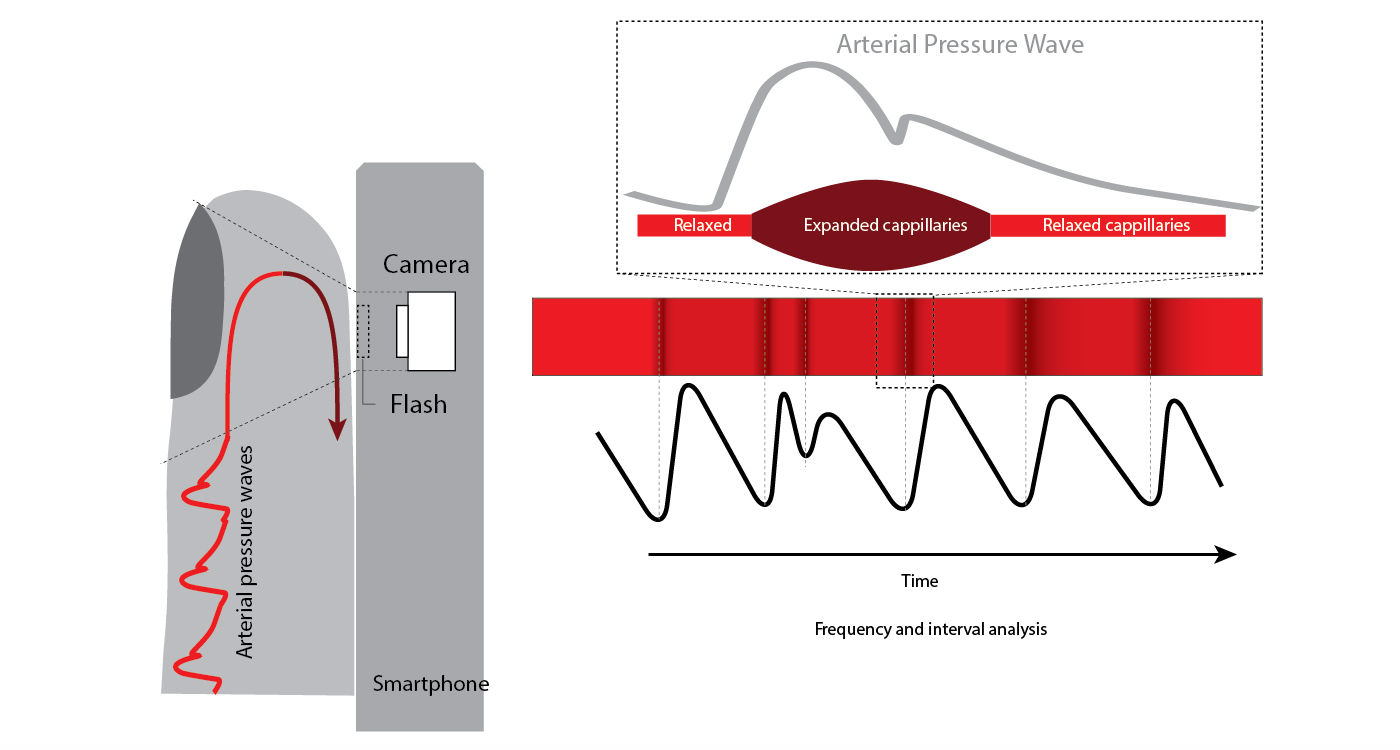
\includegraphics[width=0.5\textwidth]{PPGprinciple.jpg} 
\caption{\csentence{Recording smartphone PPG}
 While the flash illuminates the skin, the camera is recording changes in light intensity induced by tissue blood volume. \cite{Vandenberk2017}.}
 \label{fig:ppg}
\end{figure}
%%%%%%%%%%%%%%%%%%%%%%%%%%%%
PPG is an optical technique used for measuring cardiac-induced fluctuations in tissue blood volume, most commonly used at the skin surface. 
PPG requires a light source and a photoreceptor to measure fluctuations in blood volume, since blood absorbs more light than the surrounding tissue.  
The resulting PPG signal is a waveform signal that can be seen as a time series, from which characteristics of cardiac rhythm can be derived (Figure \ref{fig:ppg}). 

Theoretically, the PPG signal consists of an AC and a DC component. 
The AC component is a pulsatile waveform which relates to the fluctuations in tissue blood volume caused by the beating heart. 
The DC component is a baseline, which relates to the tissue and average blood volume of the recorded area. 
In practice however, PPG signals have a low signal-to-noise ratio (SNR), especially when collected via smartphone apps. 
PPG instrumentation is susceptible to sources of noise like the instrumentation setup, changes in environmental light, temperature, movement, breathing rate, and the tissues fat percentage \cite{Moraes2018}. 
Another problem is that the time points in the signal are unequally spaced, due to the smartphone camera not sampling at a constant rate. 
Therefore, extracting features of cardiac rhythm from PPG signals is not straightforward.

\subsection*{Analyzing raw PPG data}
Most open source algorithms for analyzing heart rhythm are designed for ECG signals, which are inherently different from PPG signals. 
As far as is known to the authors, the only open source software package for analyzing raw PPG data is \texttt{HeartPy}. 
This package is developed for analysis of physiological data in naturalistic driving experiments \cite{vanGent2019}. 
Algorithms for analyzing raw PPG data for healthcare applications are not readily available. 

We propose a method for the analysis of smartphone-obtained PPG data. 
This method needs to take into account that 1) smartphone PPG data are noisy,
and 2) that the time steps in the signal are unequally distributed. 
The ultimate objective of such a method is to yield accurate cardiovascular characteristics related to arrhythmia, e.g. heart rate and heart rate variability (HRV) measures.  
To compute accurate HRV measures, the exact location of the data points in the signal is crucial \cite{GarciaMartinez2017}.  
Therefore, it is essential to account for the unequally spaced time steps in the signal. 

The current study's focus is filtering PPG signals in order to attenuate the signal components and simultaneously reduce unwanted features (also called artefacts). 
A possible filtering method is proposed by Eilers \cite{Eilers2003}. 
This filter, called the Whittaker-Eilers (WE-) smoother is based on penalized least squares.
Cross-validation can be implemented to decide on the optimum amount of smoothing.
The unique advantage of this filter is that it can be implemented in a few lines of code and is computationally fast. 
The WE-smoother assumes uniform sampling, whereas the PPG signal is non-uniformly sampled.
Note that filtering should be applied carefully, as it can also lead to distortion of the signal and biased subsequent results \cite{Widmann2015}. 

\subsection*{The aim}
The aim of the current research report is to improve the analysis of noisy PPG signals in healthcare settings. 
In particular, we consider Whittaker-Eilers filters to increase the SNR. 
Several WE-smoothers with varying hyperparameters are applied on PPG data. 
More specifically, the impact of the non-equal time steps in the signal is assessed. 
Furthermore, the method is implemented in R, building an open source software package for analyzing noisy PPG data, called \texttt{PPGtools}. 

\section*{Implementation}
In the current study, two approaches to filter PPG data are compared. 
The first approach assumes uniform sampling whereas the second takes into account that the signal is in fact non-uniformly sampled. 
This section first discusses filtering with the WE-smoother.
Secondly, the implementation of the method in \texttt{R} \cite{RCoreTeam2019} is demonstrated.
Thirdly, the analysis strategy on how to compare the two different approaches is presented. 

\subsection*{The Whittaker-Eilers smoother}
Let  a noisy PPG signal be a series $y$ of length $m$. 
By filtering the signal, a smooth series $z$ is fit to $y$.  
The series $z$ is obtained by balancing two characteristics: lack of fit to $y$,

\begin{equation}
    S = \Sigma_i(y_i-z_i)^2
\end{equation}

and roughness of $z$,

\begin{equation}
    R = \Sigma_i(\Delta z_i)^2
\end{equation}

The WE-smoother is based on penalized least squares. The goal is to find $z$ that minimizes the penalized likelihood function: 

\begin{equation}
    Q = S \ + \lambda R
\end{equation}

where $\lambda$ is the penalty parameter. 
$Q$ can be written in matrix notation: 

\begin{equation}
    Q = |\mathbf{y - z}|^2 + \lambda|\mathbf{Dz}|^2
\end{equation}

Here, $\mathbf{D}$ is a matrix such that $\mathbf{Dz}$ is equal to $\mathbf{\Delta z}$.

\subsubsection*{Penalty parameter}
The WE-smoother penalizes the roughness of $z$. 
The higher the penalty parameter $\lambda$, the smoother $z$ will be, at a cost of a larger lack of fit to $y$. 
%For increasing $\lambda$, $z$ approaches a horizontal straight line. 

\subsubsection*{Order of the differences}
Remember that matrix $\mathbf{D}$ is a matrix such that $\mathbf{Dz}$ is equal to $\mathbf{\Delta z}$.
For a series $y$ with $m=5$,   
\[
\mathbf{D} =
  % latex table generated in R 3.6.1 by xtable 1.8-4 package
% Wed Jan  8 14:03:19 2020
\begin{bmatrix}{}
  -1 & 1 & 0 & 0 & 0 \\ 
  0 & -1 & 1 & 0 & 0 \\ 
  0 & 0 & -1 & 1 & 0 \\ 
  0 & 0 & 0 & -1 & 1 \\ 
  \end{bmatrix}
%%%%%%%%%%%%%
  \]
  


The order of differences $d$ can be varied, meaning the differences can be recursive. 
Second-order differences ($\Delta^2$) are differences between differences, and so on. 
For the series $y$ with $m=5$ and $d=2$, 

\[
\mathbf{D_2} =
% latex table generated in R 3.6.1 by xtable 1.8;4 package
% Sun Dec  8 12:50:18 2019
% latex table generated in R 3.6.1 by xtable 1.8-4 package
% Wed Jan  8 14:03:19 2020
\begin{bmatrix}{}
  1 & -2 & 1 & 0 & 0 \\ 
  0 & 1 & -2 & 1 & 0 \\ 
  0 & 0 & 1 & -2 & 1 \\ 
  \end{bmatrix}
  %%%%%%%%%%%%
  \]

\subsubsection*{Non-uniform sampling}
The WE-smoother as presented above assumes that $y$ is uniformly sampled.
To account for non-uniform sampling, the WE-smoother divides the differences in $z$ by the differences in the time points $x$, 

\begin{equation}
    g_{id} = \frac{\Delta^d z_i}{\Delta^d x_i} = \frac{z_i - z_{i-d}}{x_i - x_{i-d}}
\end{equation}

These divided differences of order $d$ are implemented in the likelihood function by a matrix $\mathbf{V}$,

\begin{equation}
Q = |\mathbf{y - z}|^2 + \lambda|\mathbf{VDz}|^2
\label{eq:likelihood}
\end{equation}

Where $\mathbf{V} = diag(1/\Delta x)$ such that $ \mathbf{VDz}$ is equal to the divided differences. 
$\mathbf{V}$ is an identity matrix if and only if the time steps in the signal are all equal to one and when $d=1$. 

\subsubsection*{Deciding on the penalty parameter}
The penalty parameter $\lambda$ can be manually tuned by visually inspecting the effect of different $\lambda$ values on $z$.  
However, a more objective evaluation of a grid of $\lambda$ values can be performed by using cross-validation. Given a series $y$ and a penalty $\lambda$, leave-one-out cross-validation can be performed.
One element of $y$ is left out, the remaining data is filtered and the left-out element is estimated ($ \hat{y}_{-i}$). 
This process can be repeated for every element in $y$. 
Now, the cross-validation standard error can be computed, which is a measure of how close the predicted values $\hat{y}$ are to the observed data $y$: 

\begin{equation}
 s_{cv} = \sqrt{{\Sigma_i (y_i - \hat{y}_{-i})}^2/m } $$
\end{equation} 

This process can be repeated the whole grid, of which the $\lambda$ with the lowest $s_{cv}$ is deemed the most optimal. 


\subsection*{Implementation in R: \texttt{PPGtools}}
The steps described in the previous section are implemented in an \verb|R|-package called \verb|PPGtools|. 
Currently under development, \verb|PPGtools| aims to provide a transparant method of analyzing noisy PPG data. 
Listing \ref{lst} provides an short demonstration of the package.
The package will be openly published on GitHub. 

\subsubsection*{Data}
The user can upload their own data, or use the demonstration PPG recording (\verb|rec|) in the package. 
The \verb|prepInput()| function takes raw PPG data and returns it as a dataframe containing only the specified time window and signal channel(s). 

\subsubsection*{Filtering} 
The core function, \texttt{smoothWE()} applies the WE-smoother on the raw signal and returns a filtered signal $z$.  
The first input argument \verb|raw_signal|, should be a raw PPG signal in the format dictated by \verb|prepInput()|. 
The function takes the following hyperparameters as remaining input: 

\begin{itemize}
\item \verb|lambda|, the desired penalty parameter $\lambda$,

\item \verb|d|, the order of differences $\Delta^d$,

\item \verb|uni|, indicating whether to assume uniform sampling (\verb|TRUE|) or account for the unequal time steps in the signal (\verb|FALSE|). 

\item \verb|cv|, indicating whether to compute the leave-one-out cross-validation standard error of this particular fit (\verb|TRUE/FALSE|).

\end{itemize}

\paragraph{Non-uniform sampling}
By default, the \verb|smoothWE()| function assumes uniform sampling.
To take into the differences in time steps, the \verb|uni| parameter can be set to \verb|FALSE|.
This parameter adds a matrix $\mathbf{V}$ to the likelihood function.

\subsubsection*{Cross-validating}
The \verb|cv| argument in the core function returns the $s_{cv}$ of the particular fit $z$. 
This enables the user to cross-validate to find optimal $\lambda$. 

\subsubsection*{Visualizing}
The \verb|plotLambda()|  function visualizes the results of smoothing with one or more $\lambda$ values. 
It plots the raw data points and the fitted data $z$ (the output of \verb|smoothWE|). 

\begin{lstlisting}[language=R, caption = Using PPGtools, label=lst]
# prepare data
raw_signal <- prepInput(data = rec, channel = "Green", tstart = 20, tstop = 40)

# fit series z
z <- smoothWE(raw_signal = raw_signal, lambda = 1, d=2, uni = TRUE, cv = FALSE)

# plot results
title <- "Uniform sampling assumed, d=2, lambda = 1"
plotLambda(raw_signal = raw_signal, z = z, title = title)
\end{lstlisting}

\subsection*{Comparison}
To demonstrate the two different approaches of the WE-smoother a PPG recording is processed twice: once with and once without the assumption of equal time steps. 
For both approaches, the workflow is as follows:
First, the effect of varying penalties $\lambda$ and order of differences $d$ is demonstrated. 
Second, the signal is filtered using a relatively high $\lambda$ value to estimate the baseline trend, which is subsequently removed from the signal. 
Third, optimal $\lambda$ values are selected using cross-validation.

At every step, the results are visually inspected.
The focus is on contrasting the two different time step approaches.
After the first step, the order of differences $d$ will be two.
In order to be able to compare the two different approaches, the time steps in the PPG signal need to be scaled. 

\section*{Results}
\subsection*{The data}
This project is part of the BigData@Heart initiative and is carried out within the Biostatistics department of the Julius Center, UMC Utrecht. 
The data consists of 15,256 anonymized PPG recordings, crowdsourced through a smartphone application called HeartforHeart. 
Active informed consent was given by the participants. 
By holding a fingertip against the camera and the LED flash, participants can ‘donate’ 90 seconds of their heart rhythm to heart research. 
This results in a signal with three colour channels. 

%%%%%%%%%%%%%%%%%%%%%%%%%%%%%%%%%%%%%%%%%%%%%%%%%%%%%%%%
%% FIGURES FOR BACKGROUND %%%%%%%%%%%%%%%%%%%%%%%%%%%%%%%%%%%%%
%%%%%%%%%%%%%%%%%%%%%%%%%%%%%%%%%%%%%%%%%%%%%%%%%%%%%%%%
%%%%%%%%%%%%%%%%%%%%%%%%%%%%%%%%%%%%%%%%%%%%%%%%%%%%%%%%
\begin{figure}[h]     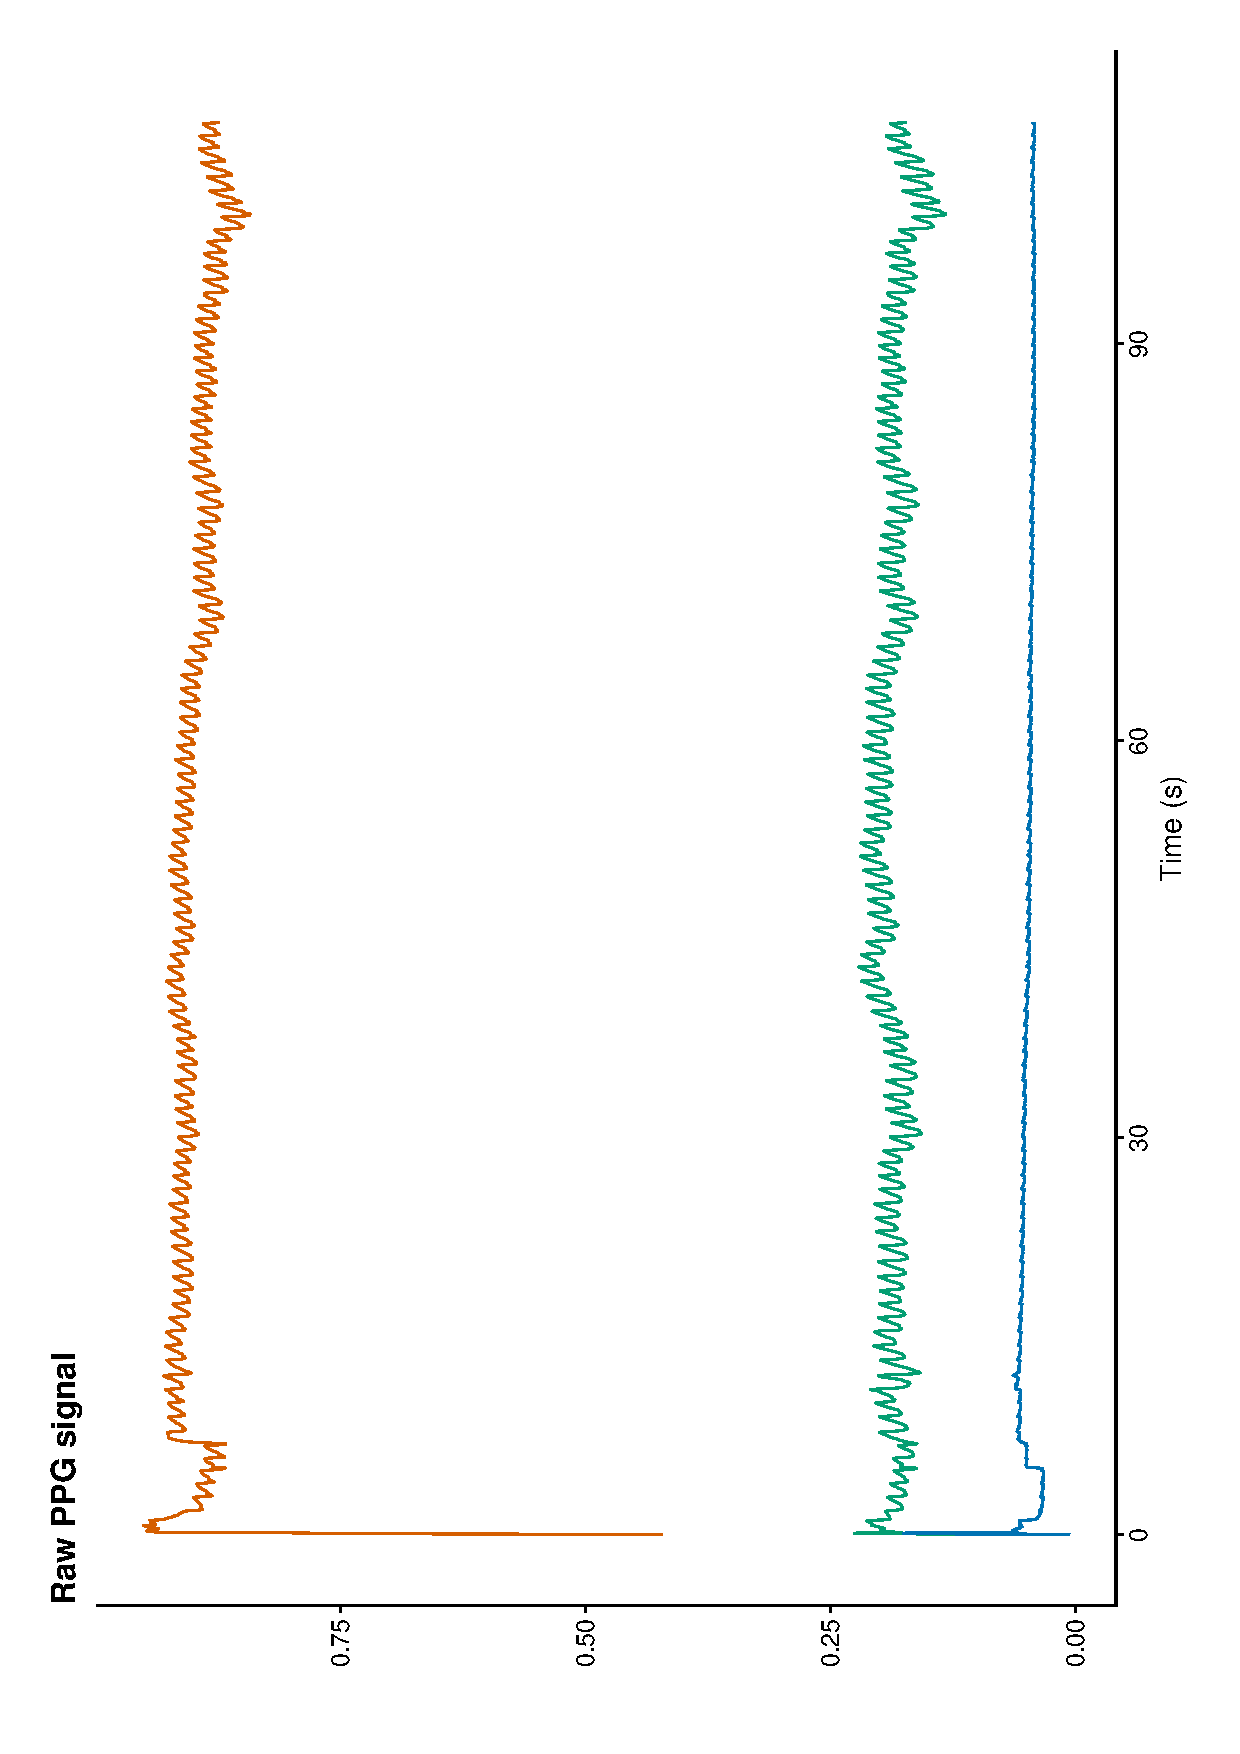
\includegraphics[height=0.4\textwidth, angle=270]{rawsignal}
    \caption{\csentence{Raw PPG signal}
    106.7 Second smartphone-obtained PPG recording. The camera recording consists of three colour channels, red, green, and blue.}
    \label{fig:rawsignal}
\end{figure}

%%%%%%%%%
\begin{figure}[h] 
    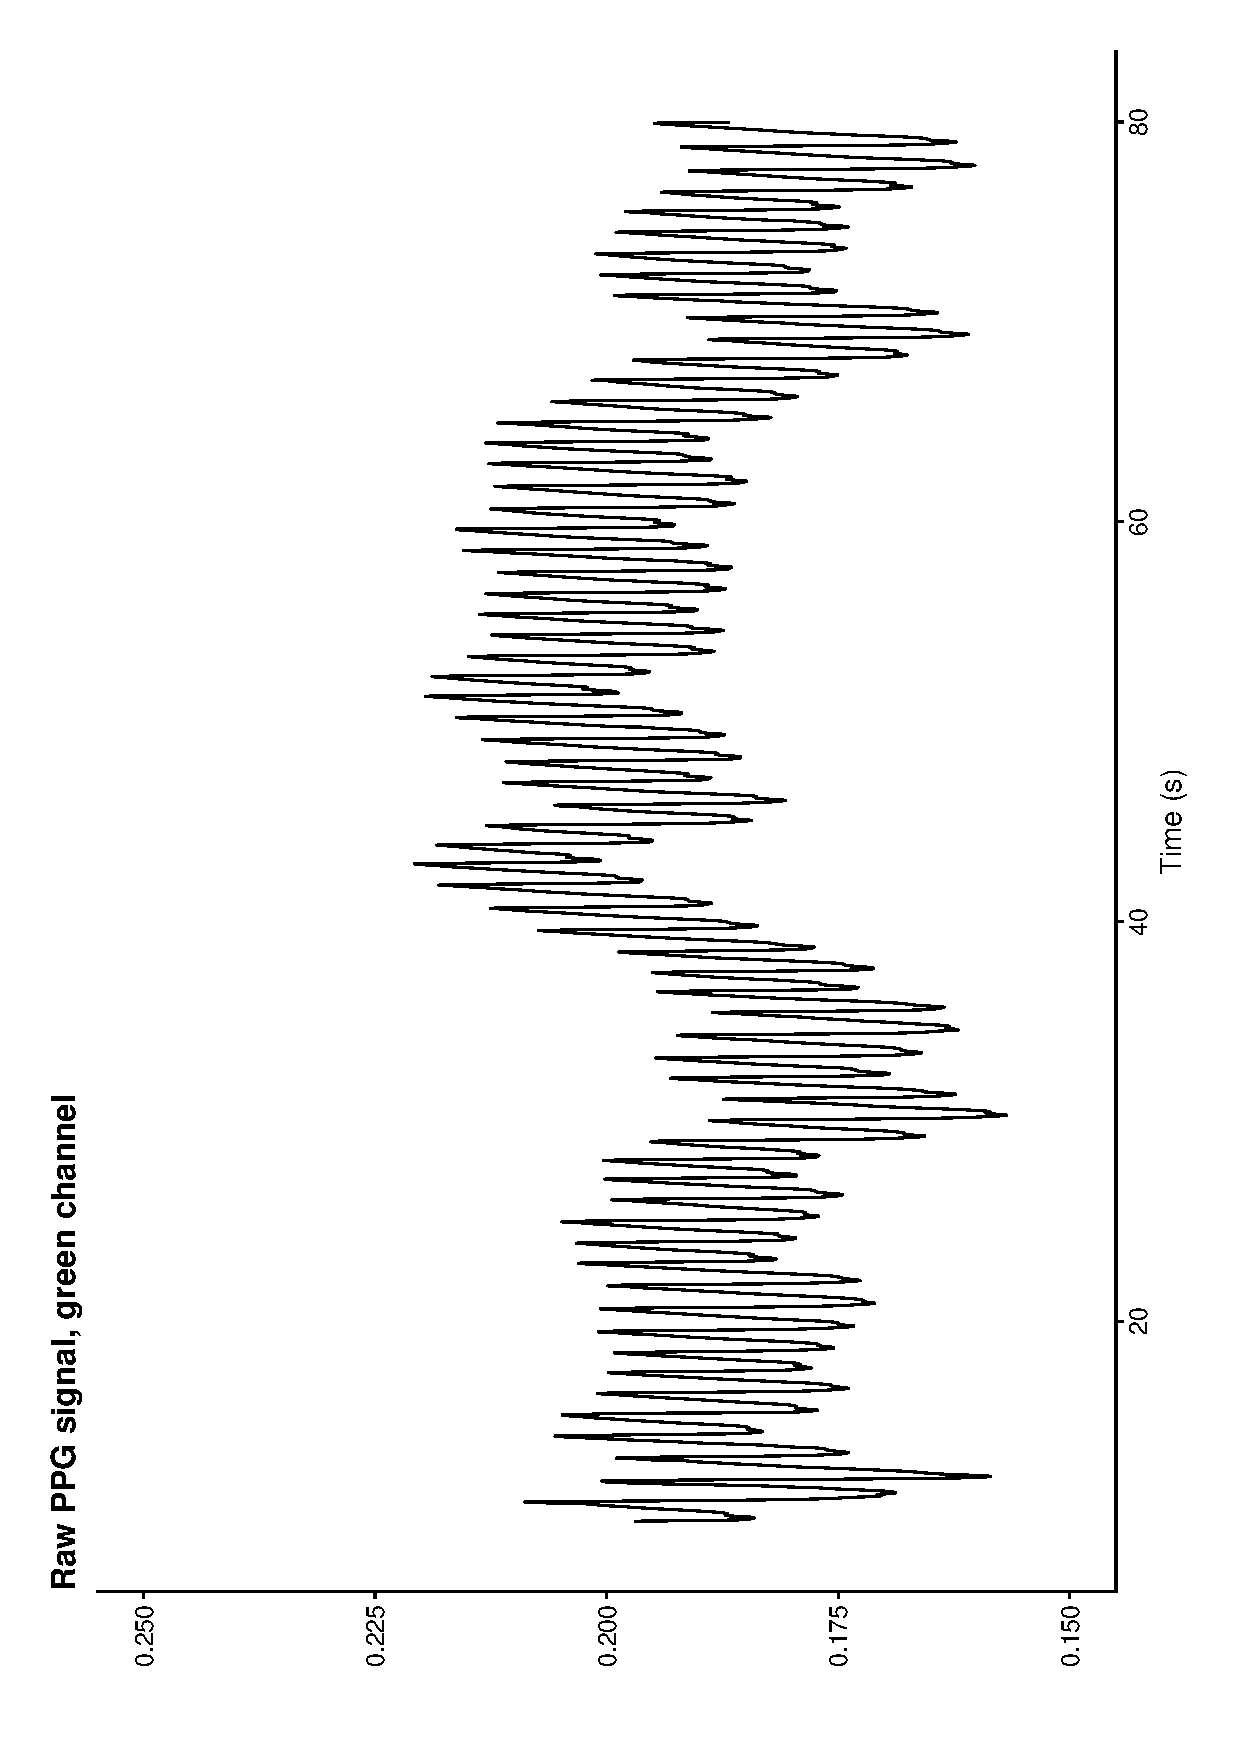
\includegraphics[height=0.4\textwidth, angle=270]{greensignal}
    \caption{\csentence{PPG-recording selected for further analysis}
    Only the green channel from the 10th to the 80th second is further processed.}
    	\label{fig:green}
\end{figure}

%%%%%%%%%%%%%%%%%%%%%%%%%%%%%%%%%%%%%%%%%%%

\subsection*{The raw signal}
The raw signal $y$ is a 106.7 seconds smartphone-obtained PPG-recording of length $m = 3200$ (Figure \ref{fig:rawsignal}).
The time points at which $y$ was sampled are in $x$. 
On average, the camera sampled at a rate of 30 frames per second (fps), with $\bar{\Delta x} = 0.033$ seconds ($s = 0.004$). The time steps ($\Delta x_i$) ranged from ranged from 0.007 to 0.089 seconds. 

For quality reasons, the green channel is selected for further processing from second 10 -- 80 (Figure \ref{fig:green}). 
As expected, the recording is a periodic signal with local maxima and minima, following the rhythm of the beating heart. 
Besides heart rhythm, the recording contains artefacts such as the fluctuating baseline of the signal, known as trend. 

\subsection*{Filtering}
\subsubsection*{Impact of $\lambda$ and $d$}
%%%%%%%%%%%%%%%%%%%%%%%%%%%%%%%%%%%%%%%%%%%%%%%%%%%%%%%
\begin{figure*}[p] 
  \begin{center}
  %%%%%%%%%%%%%%%%%%%%%%%%%%%%%%%%%%%%%%%%%%%%%%%%%%%%%%%

	\resizebox{\textwidth}{!}{
        			\subfigure[]{
			    	      \label{fig:pes1d1}
           		  	  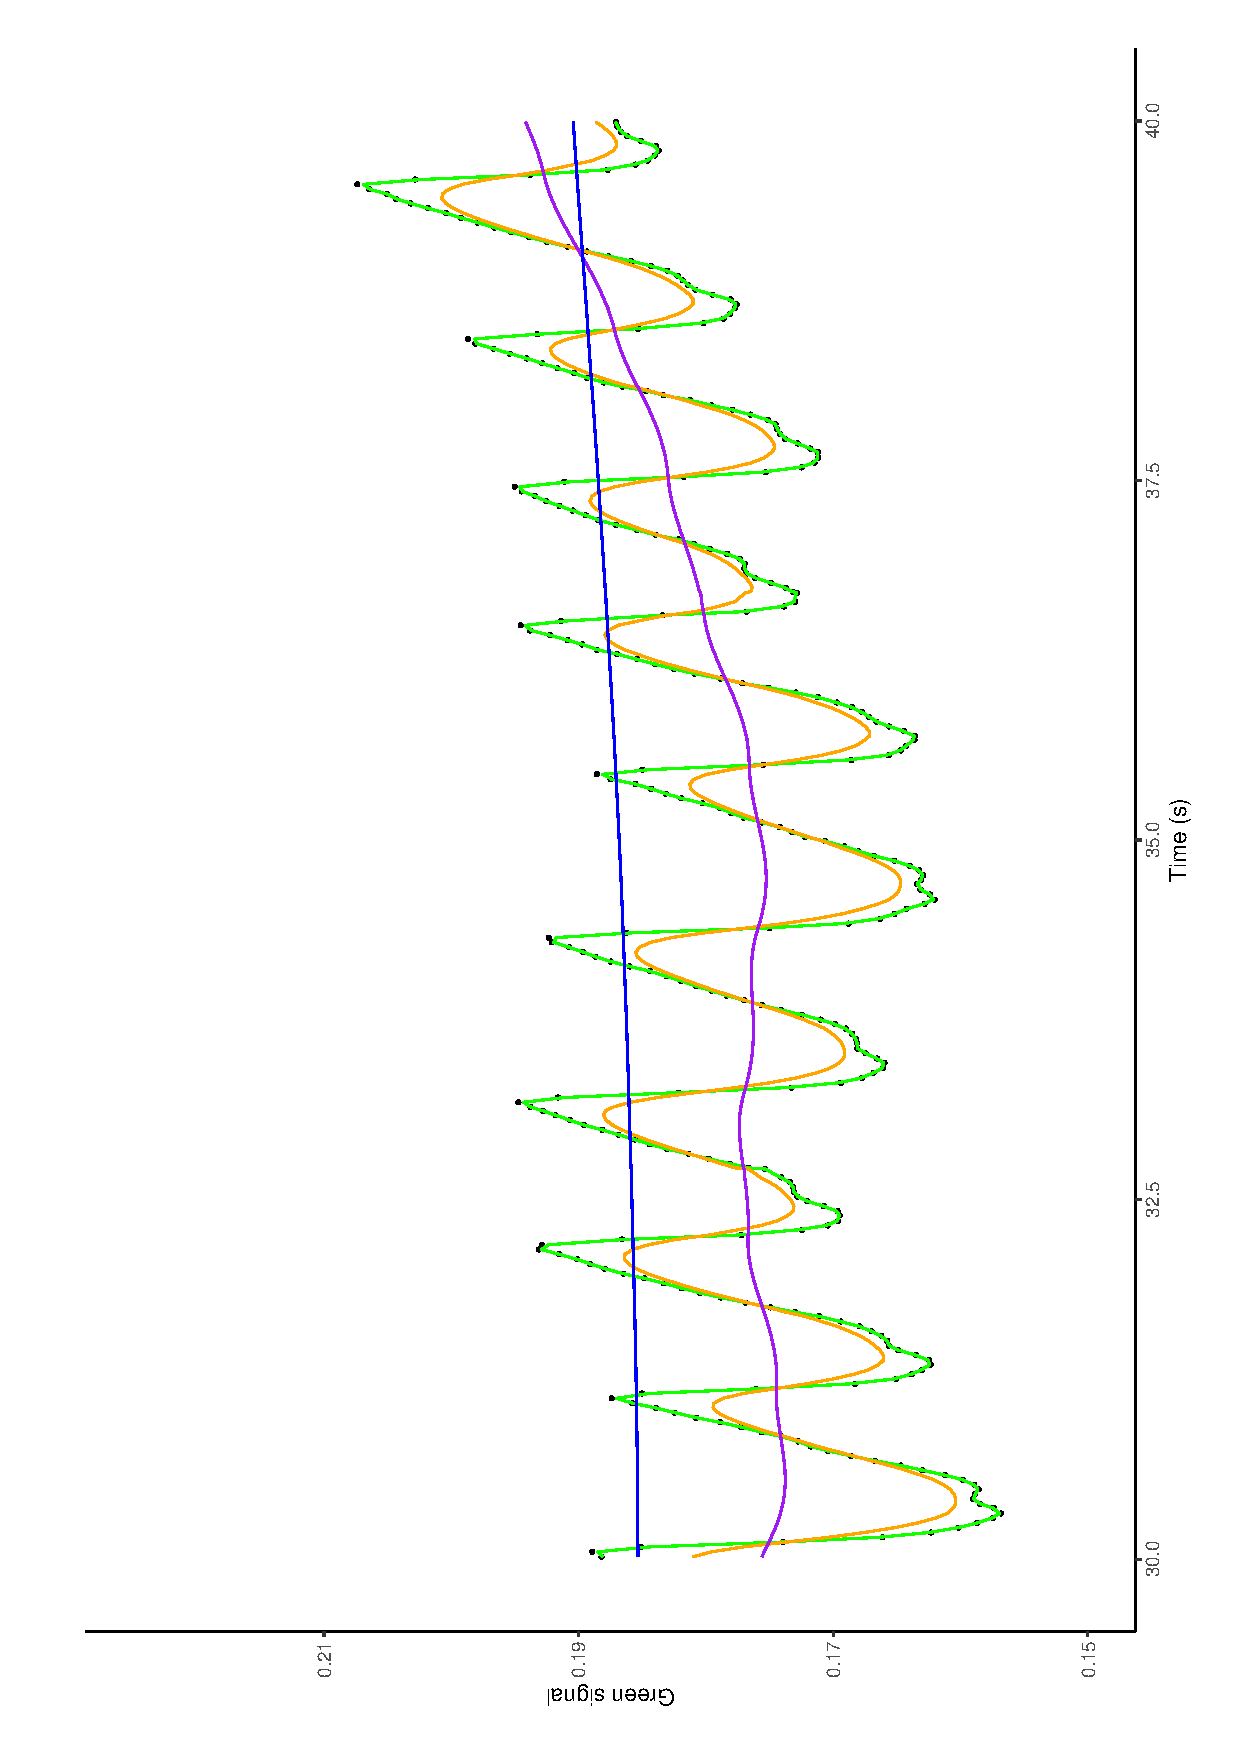
\includegraphics[width =\linewidth,angle=270]{pes1d1}
        	                 }
        			\subfigure[]{
         		            \label{fig:pues1d1}
    				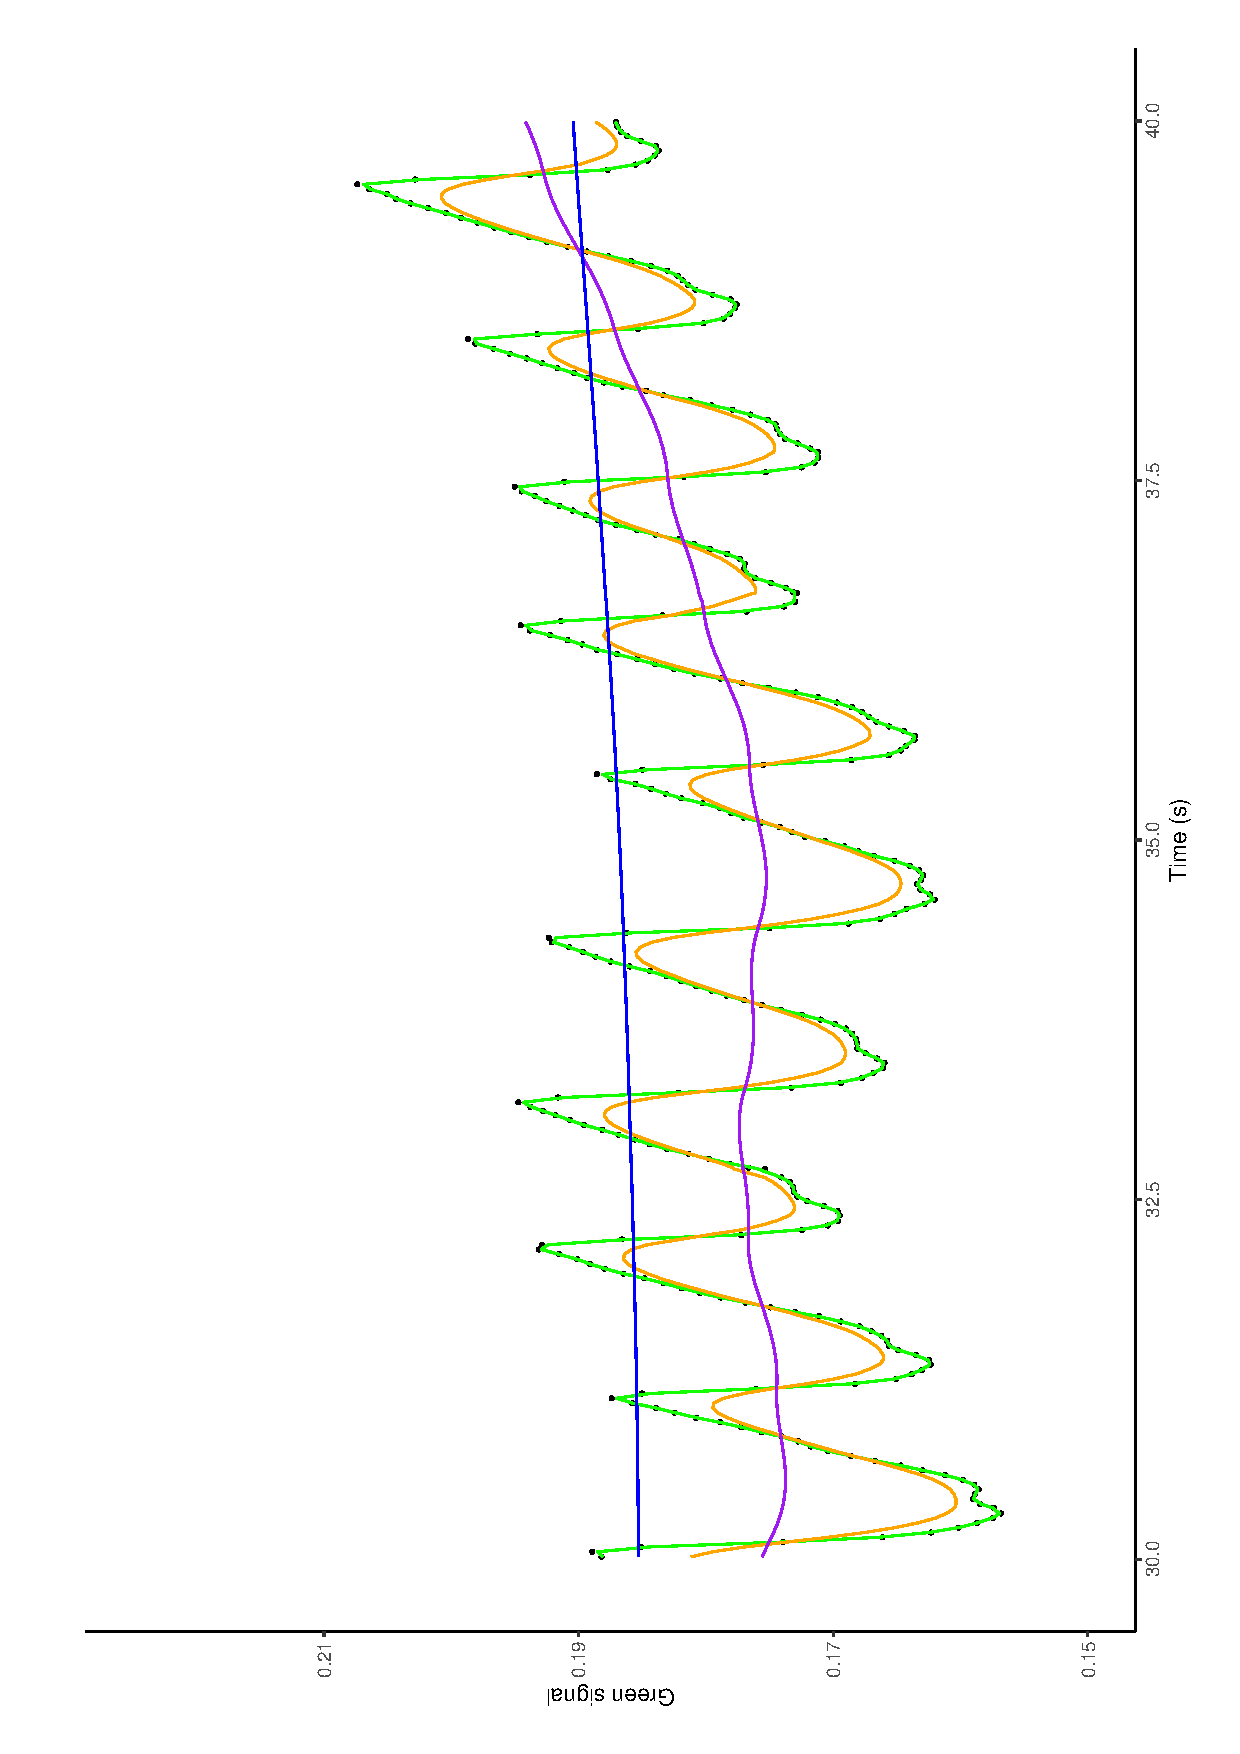
\includegraphics[width =\linewidth,angle=270]{pues1d1}
        		        }
		}\\ 	% 		
		\resizebox{\textwidth}{!}{
        			\subfigure[]{
			    	      \label{fig:pes1d2}
           		  	  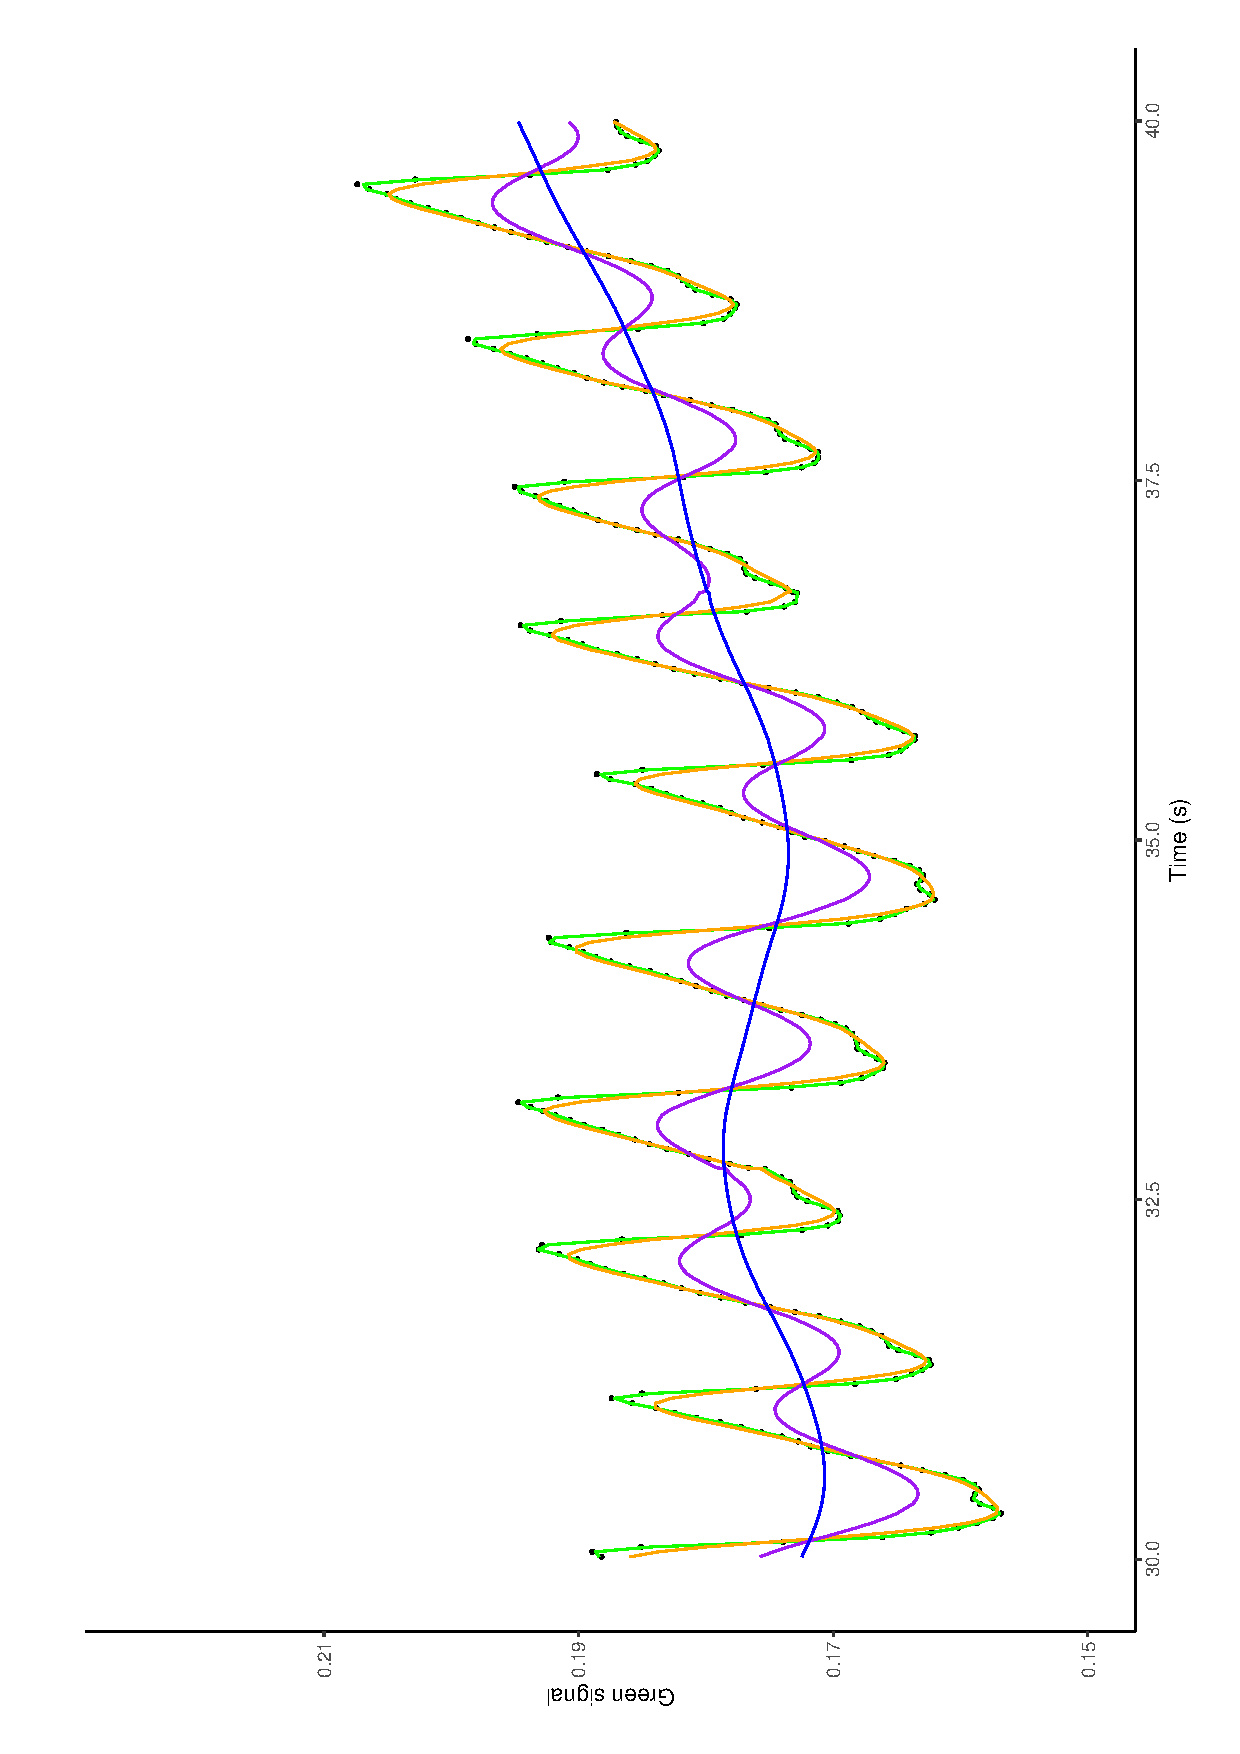
\includegraphics[width =\linewidth,angle=270]{pes1d2}
        	                 }
        			\subfigure[]{
         		            \label{fig:pues1d2}
    				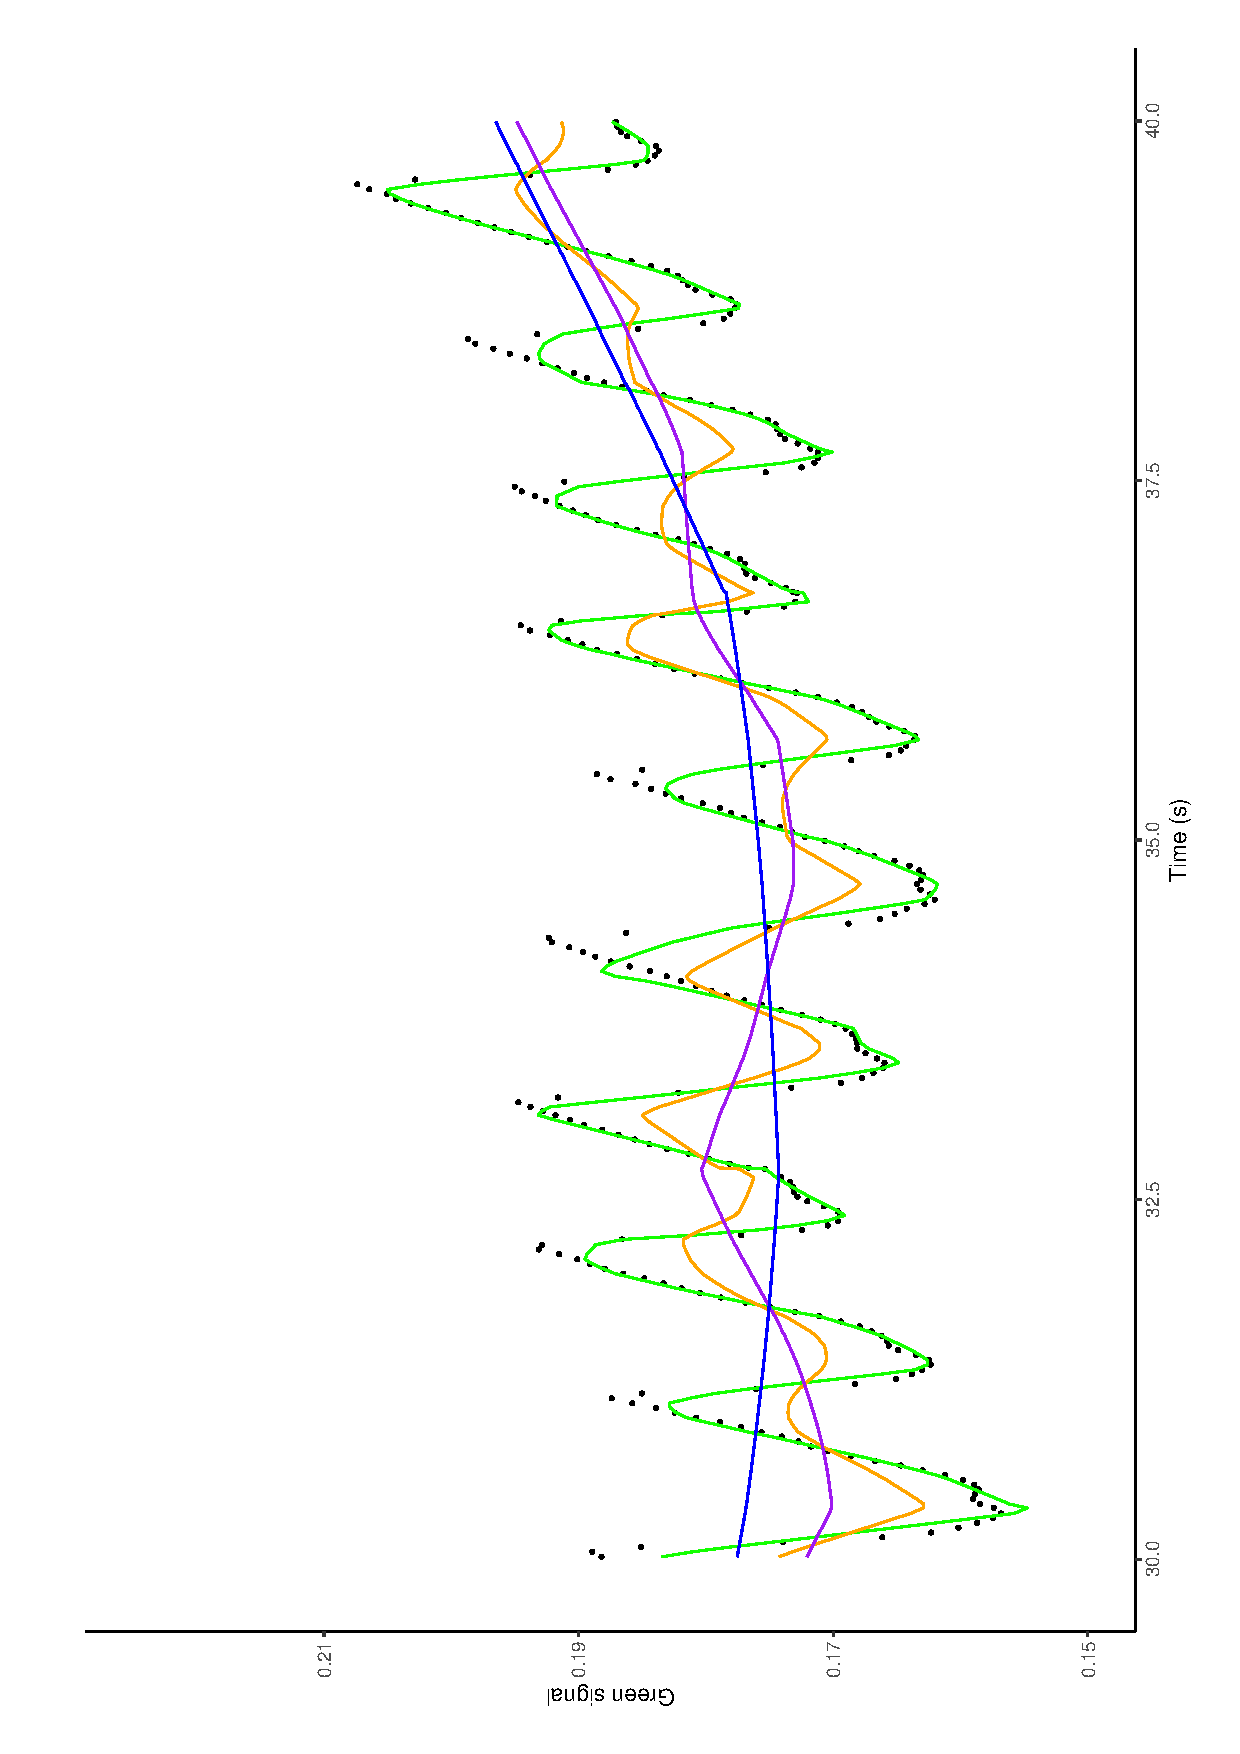
\includegraphics[width =\linewidth,angle=270]{pues1d2}
        		        }
		}\\ 	
 \resizebox{\textwidth}{!}{
        			\subfigure[]{
			    	      \label{fig:pes1d3}
           		  	  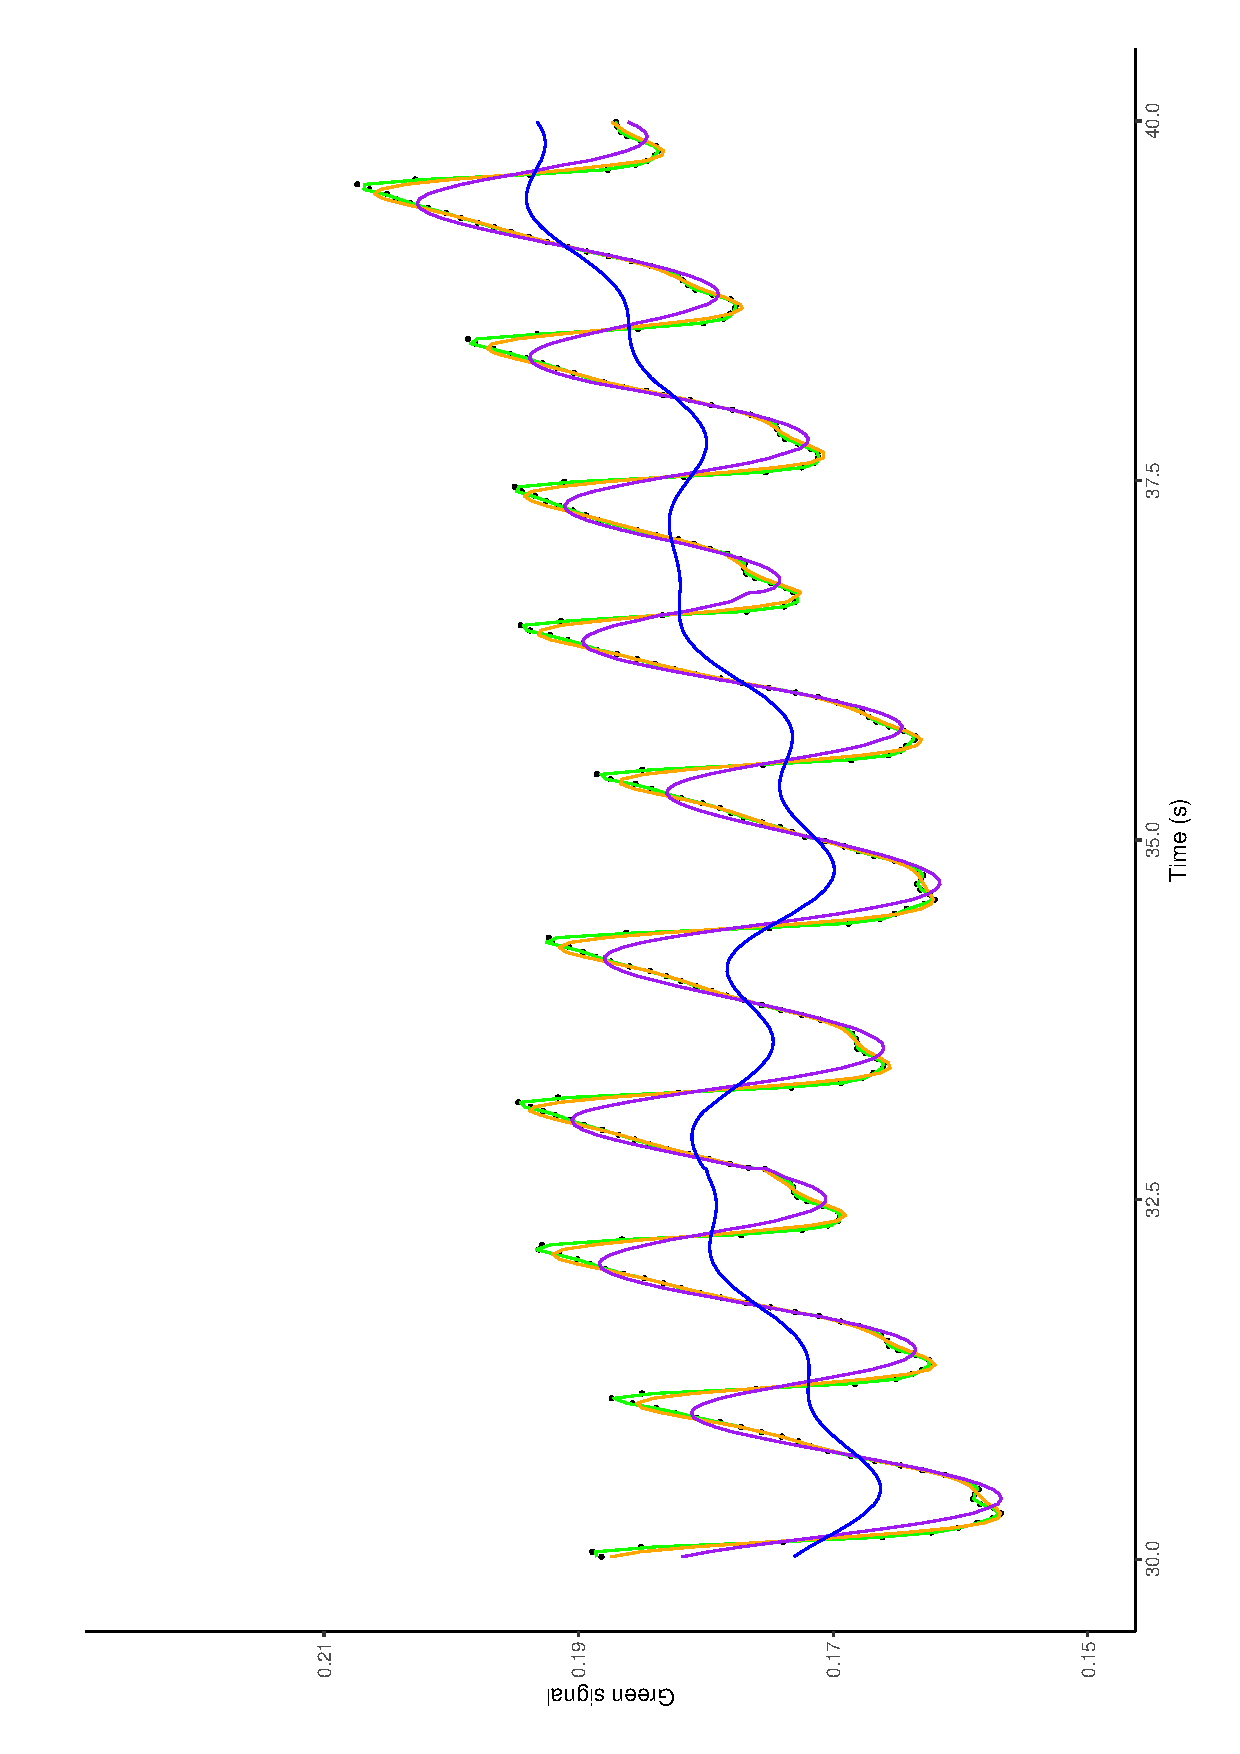
\includegraphics[width =\linewidth,angle=270]{pes1d3}
        	                 }
        			\subfigure[]{
         		            \label{fig:pues1d3}
    				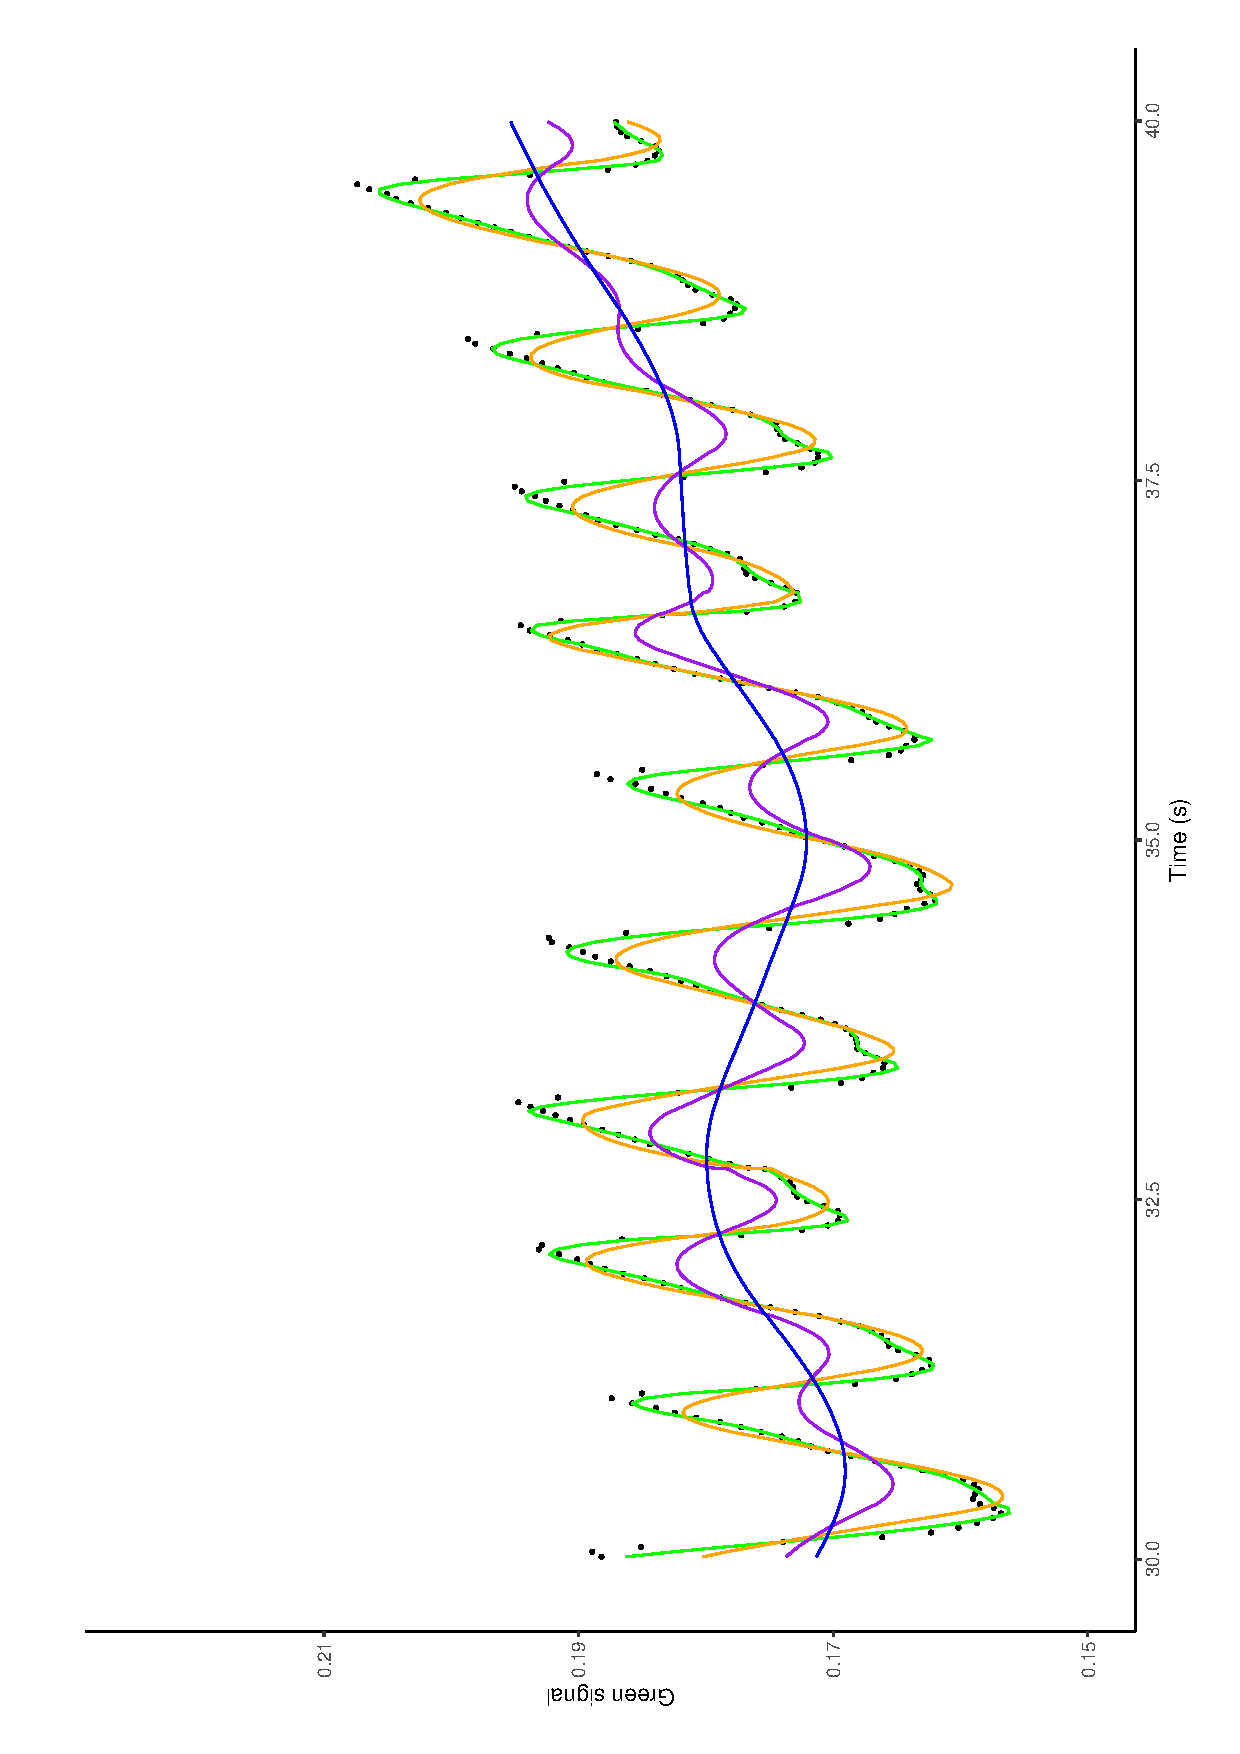
\includegraphics[width =\linewidth,angle=270]{pues1d3}
        		        }
		}\\ 	%
    %%%%%%%%%%%%%%%%%%%%%%%%%%%%%%%%%%%%%%%%%%%%%%%%%%%%%%%

     \end{center}
       	\caption{\csentence{Applying the WE-smoother on raw PPG data with different hyperparameters.} 
	In every subfigure, the raw PPG signal $y$ is represented by the black points and the fits $z$ by the coloured lines ($\lambda = \textcolor{green}{10^{-1}}, \textcolor{orange}{10^1}, \textcolor{violet}{10^3},  \textcolor{blue}{10^5}$). 
	The subfigures in the left column assume uniform sampling.
	The right column contains the results of the approach taking into account the unequal time steps.
	The remaining hyperparameters vary from from (a) - (f): (a) $\Delta ^1$, $uni = T$; (b) $\Delta ^1$, $uni = F$; (c) $\Delta ^2$, $uni = T$; (d) $\Delta ^2$, $uni = F$; (e) $\Delta ^3$, $uni = T$; (f) $\Delta ^3$, $uni = F$.}
     	  \label{fig:rawsmoothed}

\end{figure*}
%%%%%%%%%%%%%%%%%%%%%%%%%%%%%%%%%%%%%%%%%%%%%%%%%%%%%%%%
%%%%%%%%%%%%%%%%%%%%%%%%%%%%%%%%%%%%%%%%%%%%%%%%%%%%%%%

To study the impact of different hyperparameters $\lambda$ and $d$, the raw signal is filtered $4 * 3 * 2$ times: for four penalties ($\lambda = 10^{-1}, 10^1, 10^3,  10^5$),
three order differences ($d = 1, 2, 3$), 
and with and without assuming equal time steps. 

Remember that the WE-smoother penalizes the roughness of $z$. 
When accounting for unequal time steps, the roughness $\mathbf{Dz}$ is multiplied by $\mathbf{V}$. 
Therefore, the effect of a particular penalty $\lambda$ depends on whether time steps are assumed to be equal or not. 
To demonstrate this effect, five time points in the PPG signal are given 
($x = 30.82, 30.85, 30.88,  30.92, 30.95$). 
With order of differences $d = 1$, without any scaling, $\mathbf{VD}$ would look like: 
\[
\mathbf{VD} =
%%%%%%%%
% latex table generated in R 3.6.1 by xtable 1.8;4 package
% Thu Dec 12 06:58:02 2019
\begin{bmatrix}{}
  -29.41 & 29.41 & 0.00 & 0.00 & 0.00 \\ 
  0.00 & -32.33 & 32.33 & 0.00 & 0.00 \\ 
  0.00 & 0.00 & -28.45 & 28.45 & 0.00 \\ 
  0.00 & 0.00 & 0.00 & -30.02 & 30.02 \\ 
  \end{bmatrix}
  %%%%%%%%%%
\]

To scale the time points, $x$ is multiplied by the average fps of the signal.
This allows for a direct comparison of both approaches. 
When $\mathbf{V}$ would be estimated for a uniform $\Delta x$, it would be equal to identity.   
In the current signal, $\Delta x$ is non-uniform, leading to a more suitable $\mathbf{V}$ being approximately equal to identity: 

\[ 
\mathbf{VD}_{scaled} = 
% latex table generated in R 3.6.1 by xtable 1.8;4 package
% Thu Dec 12 07:27:01 2019
\begin{bmatrix}{}
  -0.98 & 0.98 & 0.00 & 0.00 & 0.00 \\ 
  0.00 & -1.08 & 1.08 & 0.00 & 0.00 \\ 
  0.00 & 0.00 & -0.95 & 0.95 & 0.00 \\ 
  0.00 & 0.00 & 0.00 & -1.00 & 1.00 \\ 
  \end{bmatrix}
\]

The 24 results of filtering the recording with varying hyperparameters are presented in Figure \ref{fig:rawsmoothed}. 
To provide enough detail, the figures only contain the 30th to the 40th second of the results.
In every hyperparameter configuration, higher $\lambda$ values led to a smoother $z$. 
In higher order differences $d$, for equal lambda values, the peaks of $z$ get closer to the peaks in the signal $y$. 
Using the unequal time steps approach, the peaks of the fit $z$ don't reach the peaks in the raw data as well as when assuming equal time steps. 
This is more extreme when using higher order differences and higher $\lambda$-values. 


\subsubsection*{Detrending}
 
 % DETRENDING PLOT 
\begin{figure*}[] 
  \begin{center}
    \resizebox{\textwidth}{!}{
			\subfigure[]{
			    	      \label{fig:dete2}
 		  	  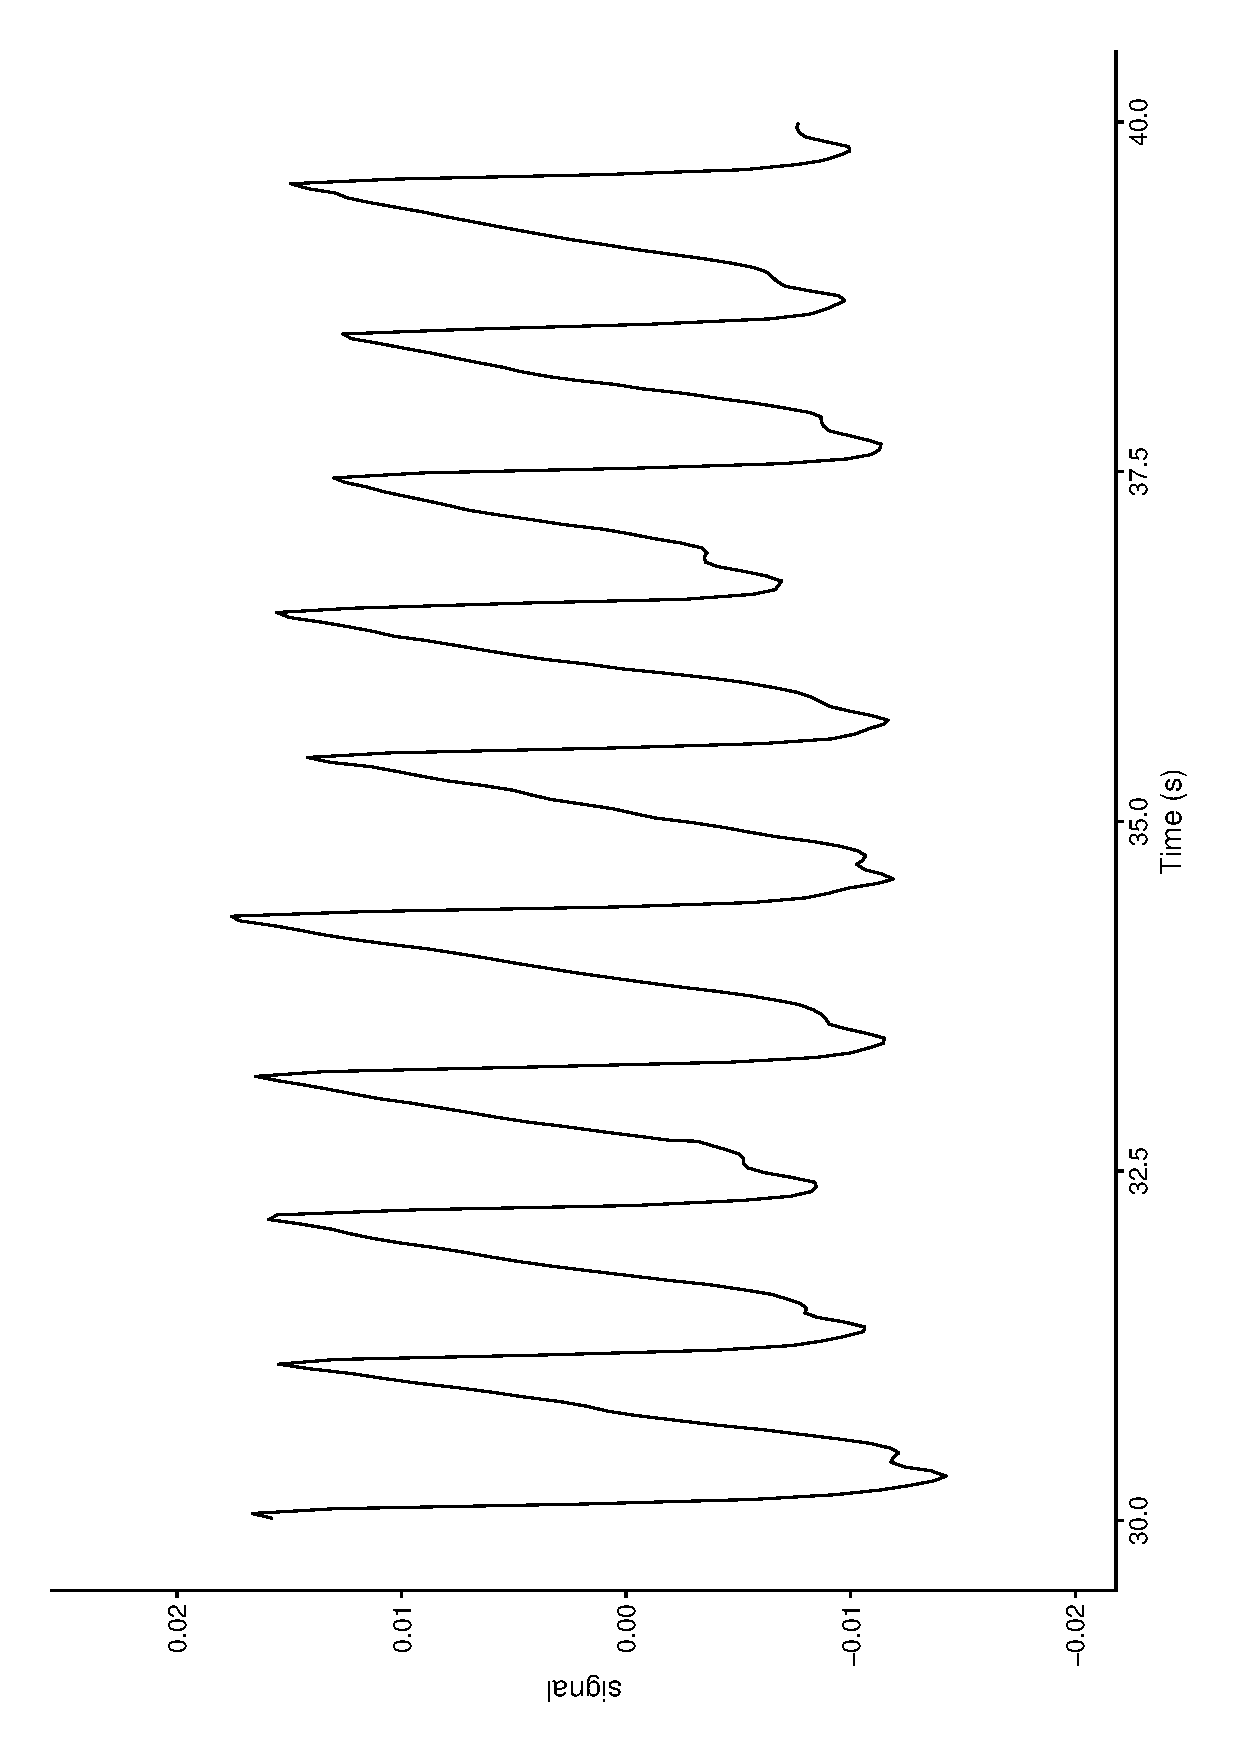
\includegraphics[angle=270, width=\linewidth]{detrended_es_d2}
	                 }
			\subfigure[]{
		            \label{fig:detu2}
				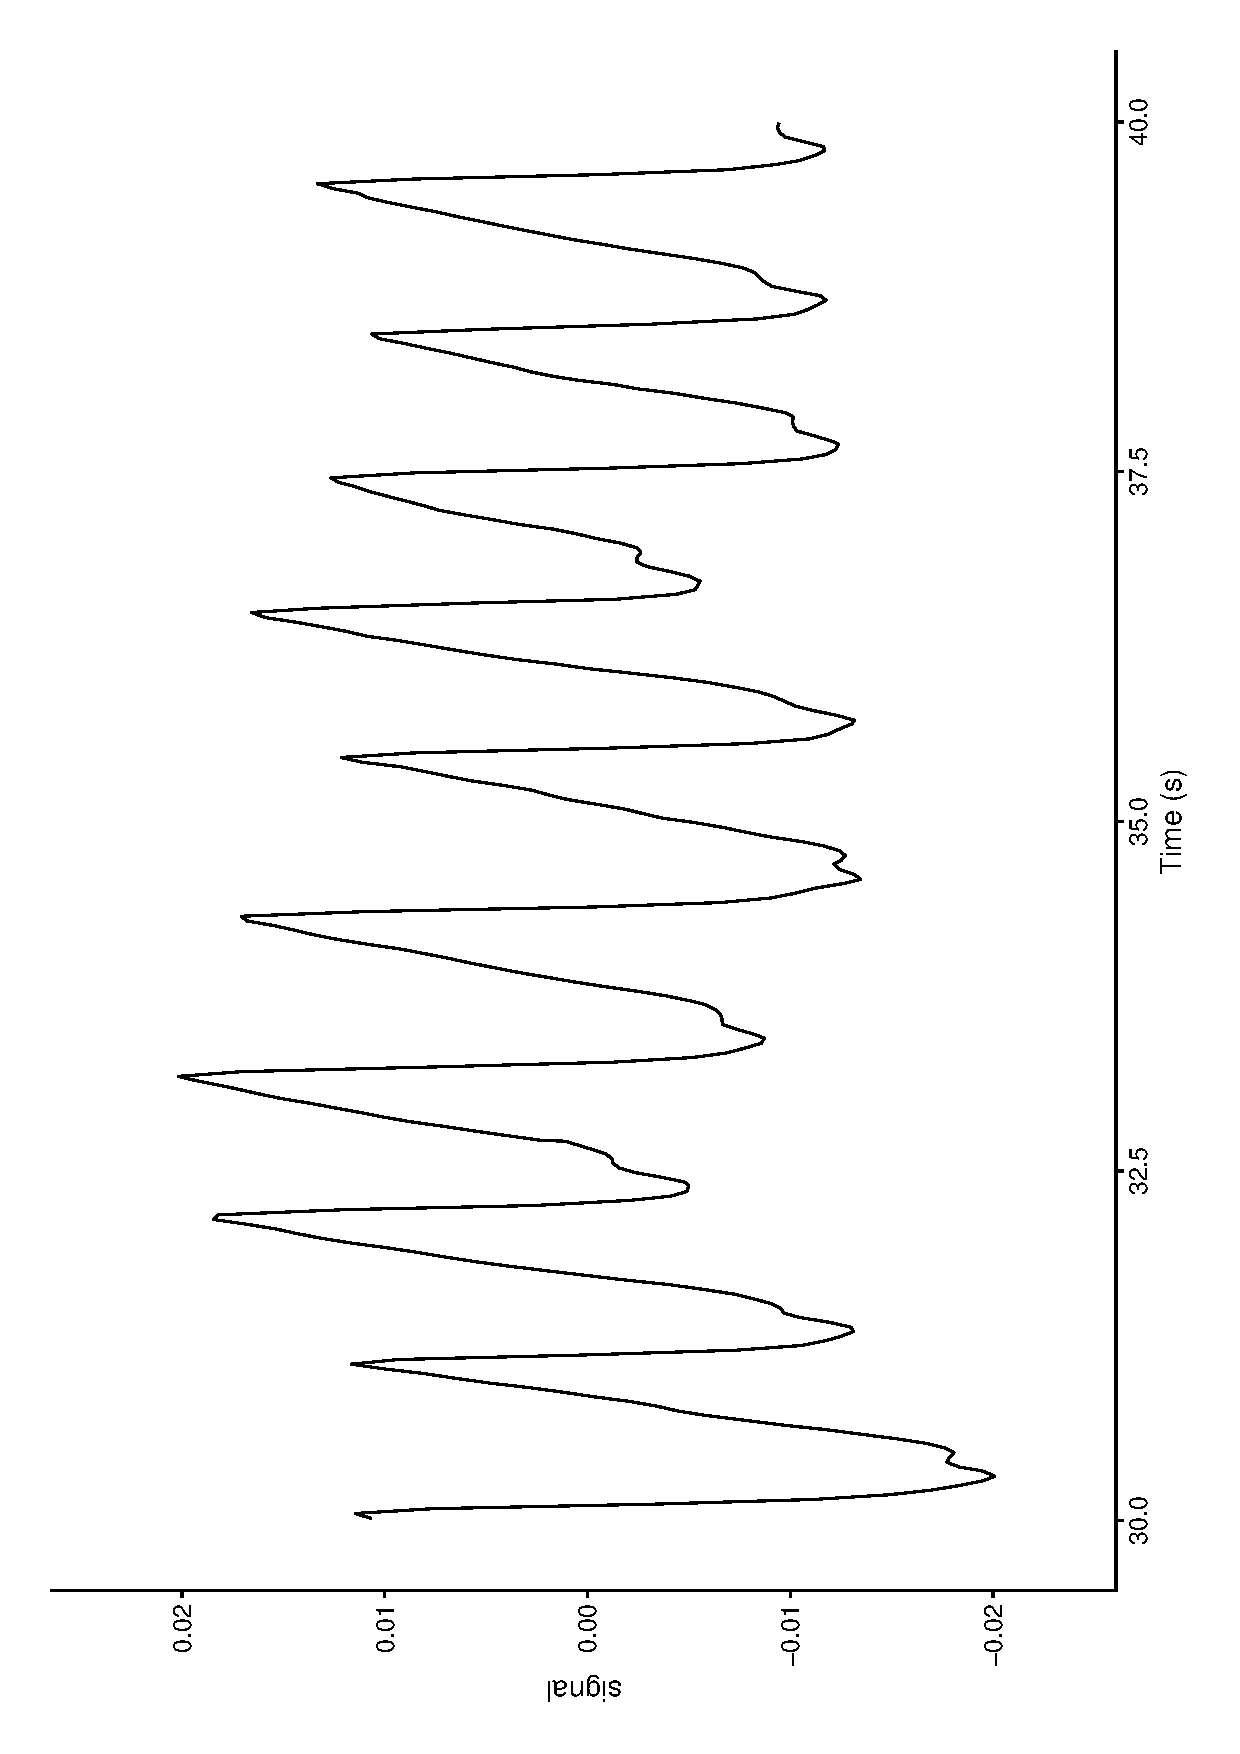
\includegraphics[angle=270, width=\linewidth]{detrended_ues_d2}
		}	% 
%%%%%%%%%%%%%%%%%%%%%%%%%%%%%%%%%%%%%%%%%%%%%%%%%%%%%%%
}
\end{center}
	\caption{\csentence{Detrended PPG data}.  
	In panel (a), the signal is detrended using the approach assuming uniform sampling.	
	Panel (b) shows the results of subtracting trend from the raw signal while accounting for non-uniform sampling.
 	Hyperparameters are constant over both approaches, $\lambda = 1000$, $\Delta^2$.}
	\label{fig:detrendedplot}
\end{figure*}

The raw data is detrended. That is, the fluctuating baseline in the signal is estimated subsequently subtracted from the raw data. 
To estimate the trend, the data is filtered with  $\lambda = 10^5$ and $\Delta ^2$ (the blue line and the second row in Figure \ref{fig:rawsmoothed}). 
Figure \ref{fig:detrendedplot} displays the detrended results. 
Compared to the raw signal, the fluctuating baseline of the detrended signal is less extreme. 
This is especially the case when uniform sampling was assumed. 

\begin{figure*}[] 
  \begin{center}
  %%%%%%%%%%%%%%%%%%%%%%%%%%%%%%%%%%%%%%%%%%%%%%%%%%%%%%%
		\resizebox{\textwidth}{!}{
        			\subfigure[]{
			    	      \label{fig:gride2}
           		  	  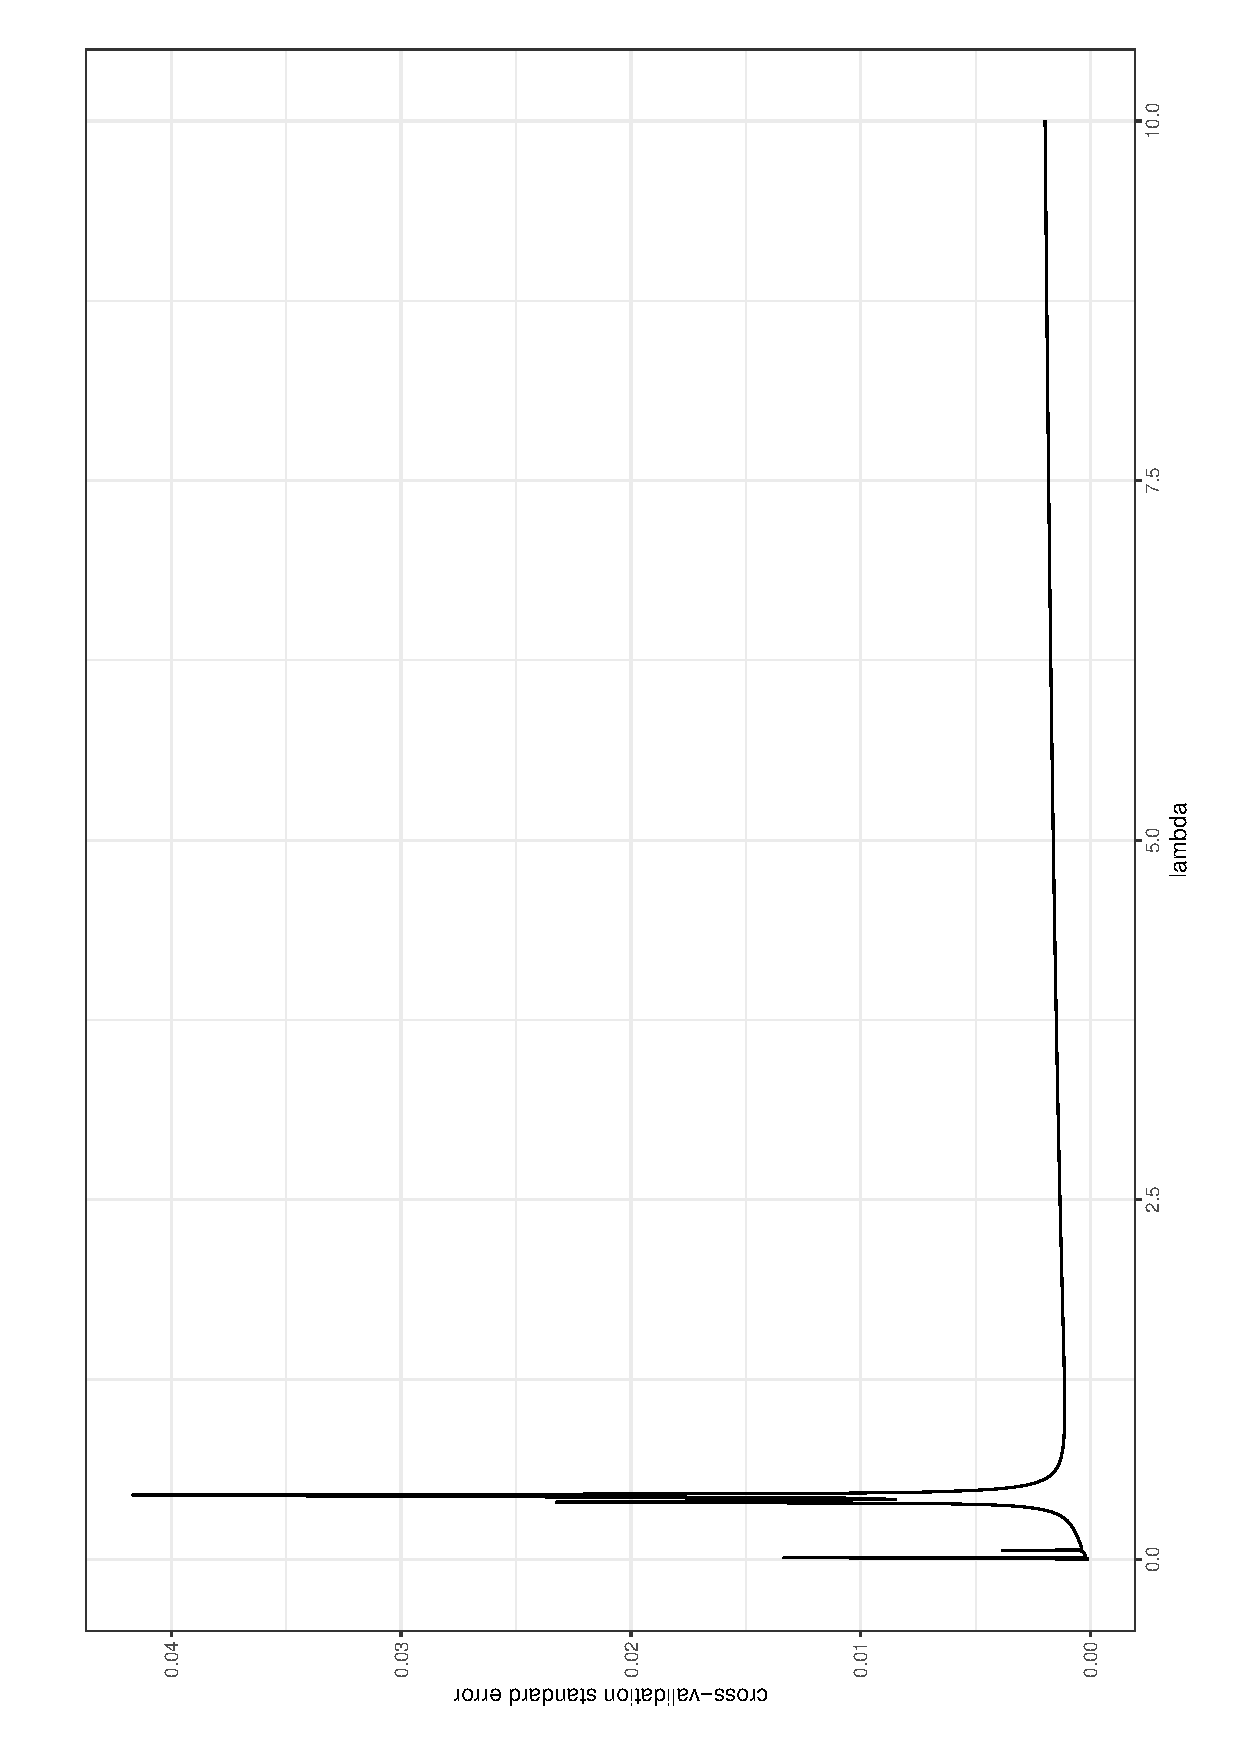
\includegraphics[angle=270, width=\linewidth]{scv_e2}
        	                 }
        			\subfigure[]{
         		            \label{fig:gridue2}
    				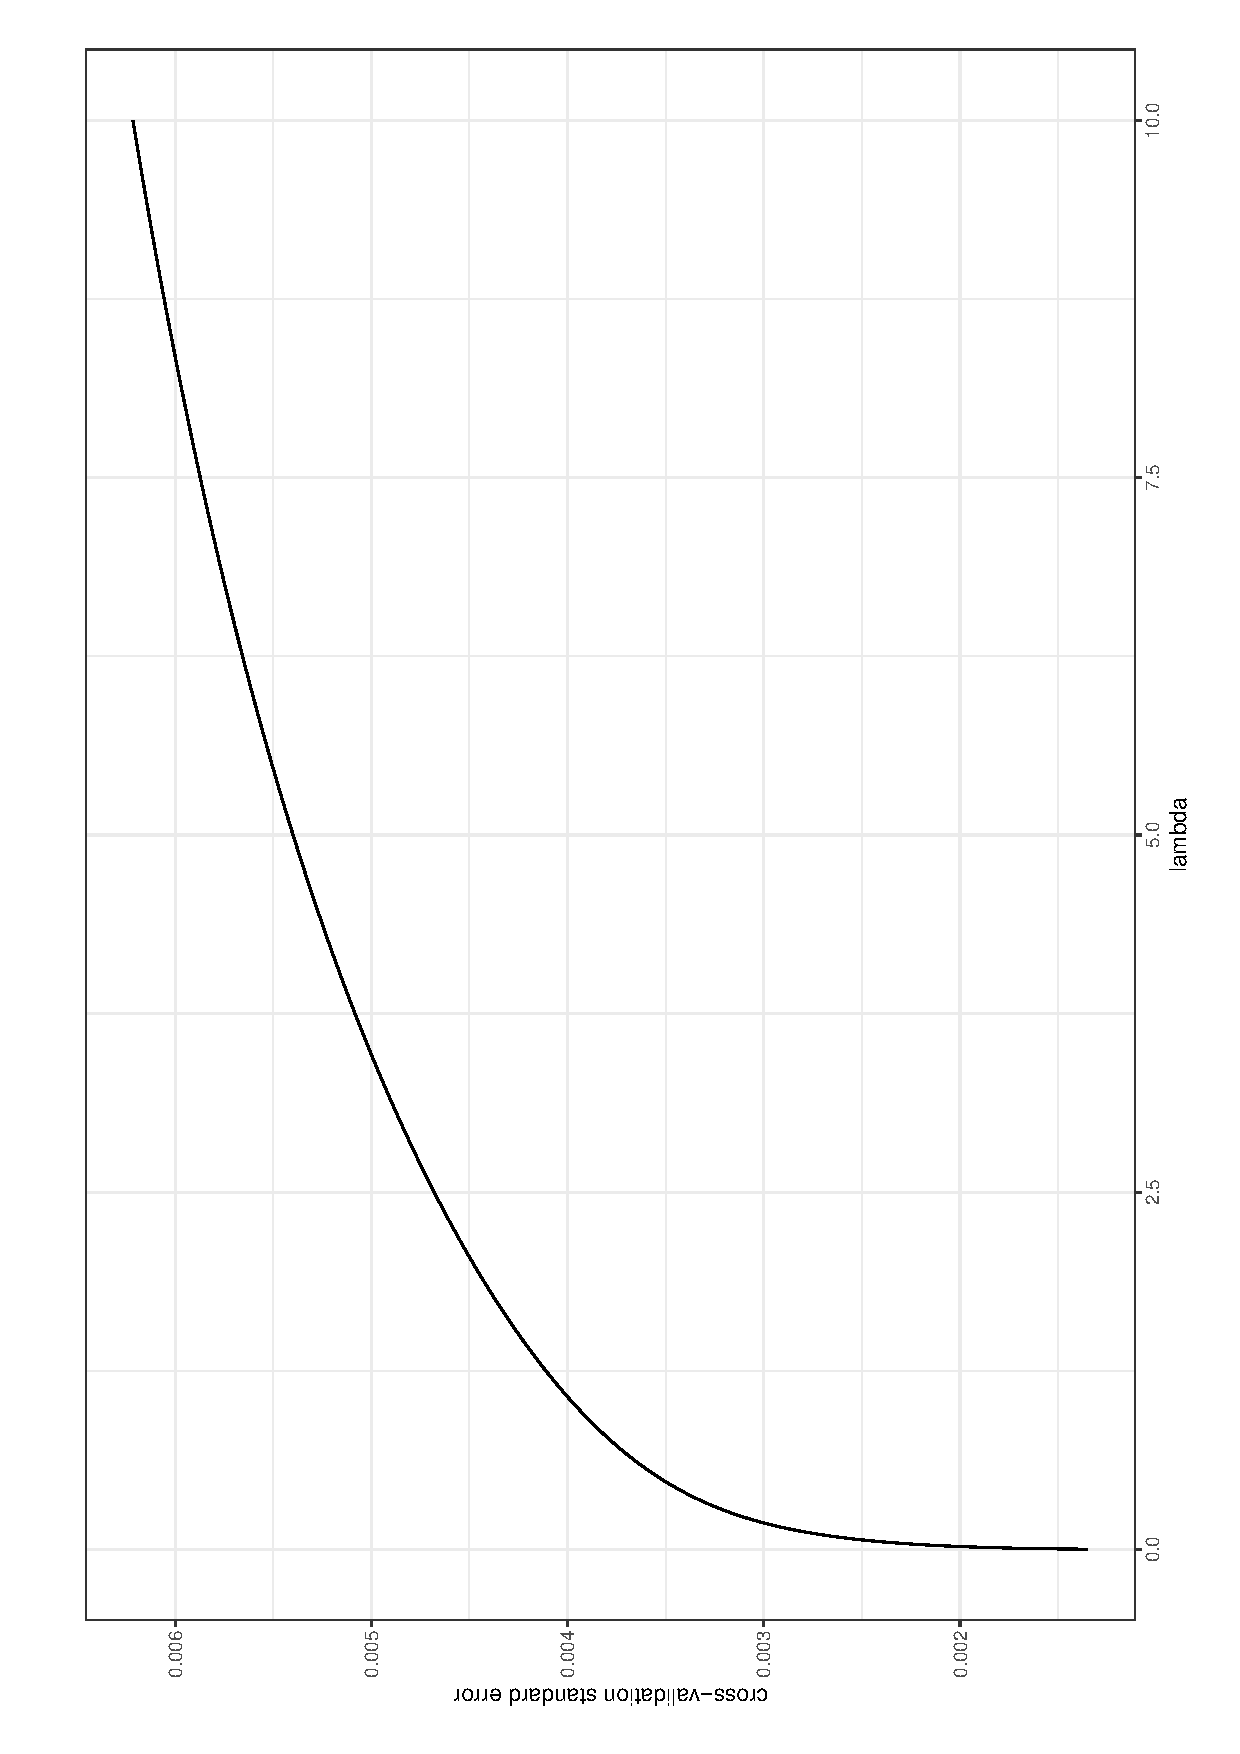
\includegraphics[angle=270, width=\linewidth]{scv_ue2}
        		        }
		}\\ 	%  

     \end{center}
       	\caption{\csentence{Grid search on detrended signal.} 
	Cross-validation standard errors were computed for a grid of $\lambda = (10^{-3}, 10^{2.99}, \dots ,10^{0.01}, 10^0)$. 
	Panel (a) shows the grid search on the detrended signal assuming uniform sampling, \ref{fig:dete2}. 
	Panel (b) shows the grid search on the detrended signal accounting for non-uniform sampling, \ref{fig:detu2}}
     	  \label{fig:gridsearch}

\end{figure*}
  %%%%%%%%%%%%%%%%%%%%%%%%%%%%%%%%%%%%%%%%%%%%%%%%%%%%%%%

\subsubsection*{Filtering with optimal $\lambda$ values}
The detrended signal is filtered again, this time with a relatively small $\lambda$ value in order to remove low-frequency noise. 
To select optimal penalty, a search is performed on the grid $\lambda = (10^{-3}, 10^{2.99}, \dots ,10^{0.01}, 10^0)$ 
See Figure \ref{fig:gridsearch} for the results. 
When assuming equal time steps, the minimum $s_{cv} = 0.0001166675$ and occurs at $\lambda = 0.001819701$.
The pattern of the grid search is highly irregular (Figure \ref{fig:gride2}).
When taking into account the unequal time steps, the minimum $s_{cv} = 0.00134817$ and occurs at $\lambda = 0.001$, the smallest $\lambda$ used in the search.
Here, the grid search \ref{fig:gridue2} shows that the $s_{cv}$ goes down as $\lambda$ approaches zero. 


\section*{Discussion} 
The current study aimed to contribute to a transparent method for analyzing noisy PPG signals in healthcare settings. 
Several WE-smoothers were applied to a noisy PPG signal in order to increase SNR. 
The main focus was comparing the performance of two filtering approaches. 
The first approach assumed uniform sampling, the second approach accounted for non-uniform sampling.
Accounting for non-uniform sampling was possible by using divided differences instead of differences in $z$ only.
Besides exploring the impact of several WE-filters, the study considered removing trend from the raw signal and cross-validating to find the optimal penalty parameter. 
\verb|PPGtools| was developed to facilitate transparant analysis of raw PPG-signals.   
At the moment, the package offers a toolbox for filtering noisy PPG signals using the WE-smoother. 
Moreover, it contains the option to cross-validate to find the optimal penalty parameter and functions for visualizing the results.

Visual inspection led to the conclusion that the WE-smoother is a suitable method to estimate and subsequently remove trend from PPG-signals. 
It seems that filtering the raw signal using the unequal time steps approach performs worse in terms of visual fit to the observed signal, except for first order differences where both approaches seemed to fit equally well. 
This is at least partially due to the chosen hyperparameters. 
In higher-order differences, the same penalty has a disproportional impact on the unequal time steps approach.
Following the discussion about adding matrix $\mathbf{V}$ to account for unequal time steps, it can be concluded that the two approaches are penalizing roughnesses that are inherently different and therefore cannot be directly compared. 
The solution was to scale the time points such that when time steps are unequal, $\mathbf{V}$ is approximately equal to an identity matrix.
However, this does not hold when using higher order differences. 
Therefore, the current scaling approach only allows for a fair comparison between the two approaches when using order differences. 
Further research is needed to obtain a proper matrix $\mathbf{V}$ for any choice of $d$. 

In both approaches, cross-validation for $\lambda$ was performed. 
When assuming uniform sampling, cross-validation lead to heavily fluctuating $s_{cv}$ over a grid of $\lambda$-values.
To explain the unexpected fluctuations, the cross-validation method has to be evaluated in more detail. 
When accounting for non-uniform sampling, cross-validation suggests minimum smoothing. 
Since a PPG-signal is periodic, the errors of the fit $z$ will be dependent on $x$. 
Therefore, the $\lambda$ value with the lowest $s_{cv}$ will be the one where smoothing is minimal, e.g. the lowest $\lambda$ value. 
From this result we conclude that the current cross-validation approach is possibly not the most suitable for periodic signals.
Therefore, further research into cross-validation methods other than leave-one-out is needed. 

\section*{Conclusions}
The study was of an explorative nature and yielded insight in the impact of the WE-smoother on noisy PPG data.
This resulted in many pointers to next steps to take. 
Finding a fair comparison method for the approaches assuming equal time steps versus accounting for unequal steps is of primary concern
Secondary, the method of finding the optimal penalty parameter using cross-validation needs further investigation. 
After that, the method can be further extended with the extraction of heart rate characteristics. 
These steps should continue to contribute to a transparent method of analyzing noisy PPG signals, implemented in \verb|PPGtools|. 

%%%%%%%%%%%%%%%%%%%%%%%%%%%%%%%%%%%%%%%%%%%%%%
%%                                          %%
%% Backmatter begins here                   %%
%%                                          %%
%%%%%%%%%%%%%%%%%%%%%%%%%%%%%%%%%%%%%%%%%%%%%%

\begin{backmatter}

%%%%%%%%%%%%%%%%%%%%%%%%%%%%%%%%%%%%%%%%%%%%%%%%%%%%%%%%%%%%%
%%                  The Bibliography                       %%
%%                                                         %%
%%  Bmc_mathpys.bst  will be used to                       %%
%%  create a .BBL file for submission.                     %%
%%  After submission of the .TEX file,                     %%
%%  you will be prompted to submit your .BBL file.         %%
%%                                                         %%
%%                                                         %%
%%  Note that the displayed Bibliography will not          %%
%%  necessarily be rendered by Latex exactly as specified  %%
%%  in the online Instructions for Authors.                %%
%%                                                         %%
%%%%%%%%%%%%%%%%%%%%%%%%%%%%%%%%%%%%%%%%%%%%%%%%%%%%%%%%%%%%%

% if your bibliography is in bibtex format, use those commands:

\bibliographystyle{bmc-mathphys} % Style BST file (bmc;mathphys, vancouver, spbasic).
\bibliography{thesisPPG_Gerbrich.bib}    % Bibliography file (usually '*.bib' )

% for author;year bibliography (bmc;mathphys or spbasic)
% a) write to bib file (bmc;mathphys only)
% @settings{label, options="nameyear"}
% b) uncomment next line
%\nocite{label}

% or include bibliography directly:
% \begin{thebibliography}
% \bibitem{b1}
% \end{thebibliography}

%%%%%%%%%%%%%%%%%%%%%%%%%%%%%%%%%%%
%%                               %%
%% Figures                       %%
%%                               %%
%% NB: this is for captions and  %%
%% Titles. All graphics must be  %%
%% submitted separately and NOT  %%
%% included in the Tex document  %%
%%                               %%
%%%%%%%%%%%%%%%%%%%%%%%%%%%%%%%%%%%

%%
%% Do not use \listoffigures as most will included as separate files
%
%\section*{Figures}
%

%%%%%%%%%%%%%%%%%%%%%%%%%%%%%%%%%%%
%%                               %%
%% Tables                        %%
%%                               %%
%%%%%%%%%%%%%%%%%%%%%%%%%%%%%%%%%%%

%% Use of \listoftables is discouraged.
%%
%\section*{Tables}
%\begin{table}[h!]
%\caption{Sample table title. This is where the description of the table should go.}
%      \begin{tabular}{cccc}
%        \hline
%           & B1  &B2   & B3\\ \hline
%        A1 & 0.1 & 0.2 & 0.3\\
%        A2 & ... & ..  & .\\
%        A3 & ..  & .   & .\\ \hline
%      \end{tabular}
%\end{table}

%%%%%%%%%%%%%%%%%%%%%%%%%%%%%%%%%%%
%%                               %%
%% Additional Files              %%
%%                               %%
%%%%%%%%%%%%%%%%%%%%%%%%%%%%%%%%%%%

%\section*{Additional Files}
%  \subsection*{Additional file 1 ;;; Sample additional file title}
%    Additional file descriptions text (including details of how to
%    view the file, if it is in a non;standard format or the file extension).  This might
%    refer to a multi;page table or a figure.
%
%  \subsection*{Additional file 2 ;;; Sample additional file title}
%    Additional file descriptions text.


\end{backmatter}
\end{document}


%%%%%%%%%%%%%%%%%%%%%%%% the end % 
